
\clearpage

\section {Results of the $\bar{\nu}/\nu$ joint analysis with the Run 1-7b dataset}
\label{sec:results_run17b}

The results of the Run 1-7b data set fit,
for an exposure 
of \TotalPotNuRunOneSevenB POT in neutrino mode
and
of \TotalPotNuBarRunOneSevenB POT in antineutrino mode, 
are shown in this chapter.
In \cref{fig:spectra_expVsdata_asimov_A_run17b} the predicted spectra of $\mu$-like and $e$-like samples
are compared to the observed data.
In \cref{tab:num_events_run17b} the expected and observed number of events in Run 1-7b data set are shown.
The predicted number of events are shown for the oscillation parameters in \cref{tab:osc_params_joint_asimov}
of Asimov data sets A and B.
%All the predicted and observed events are in good agreement.

Compared to Run 1-6 data set one more event both in neutrino and antineutrino mode $e$-like is observed
and the event rate is still compatible with $\delta_{CP} = -\pi/2$.
The neutrino mode $\mu$-like sample got only one more event from Run 1-7b
while the antineutrino mode $\mu$-like sample has about double of the statistic.

The comparison of the confidence intervals obtained by the fit of the Run 1-7b data set
among all the oscillation analysis groups is shown in \cite{Mach3JointFitRun16}.

\begin{figure}
\center
\begin{subfigure}[b]{0.49\textwidth}
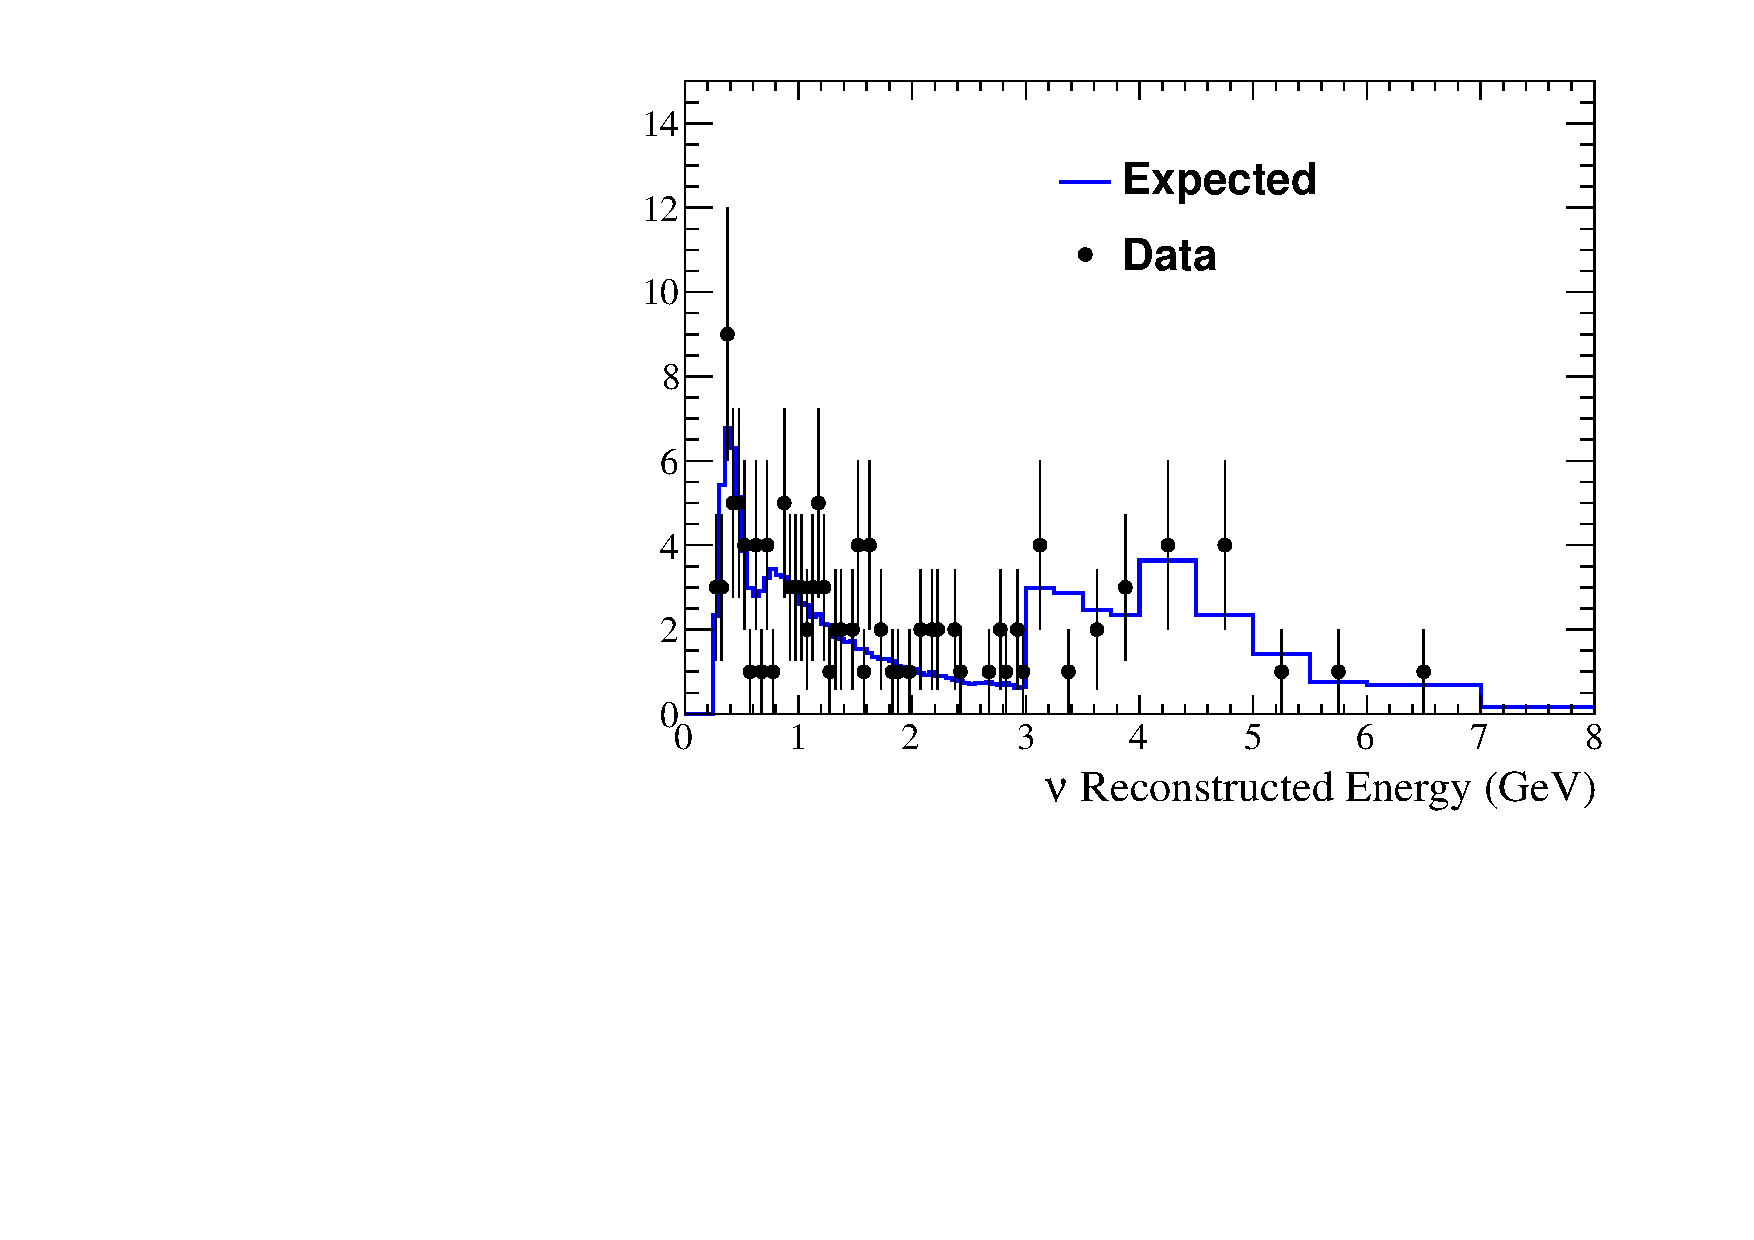
\includegraphics[width=0.9\textwidth]{./joint_plots/data/Run17b/spectrum_data_exp_1Rmu_Run17.pdf}
\caption{Muon-like, neutrino mode}
\end{subfigure}
\begin{subfigure}[b]{0.49\textwidth}
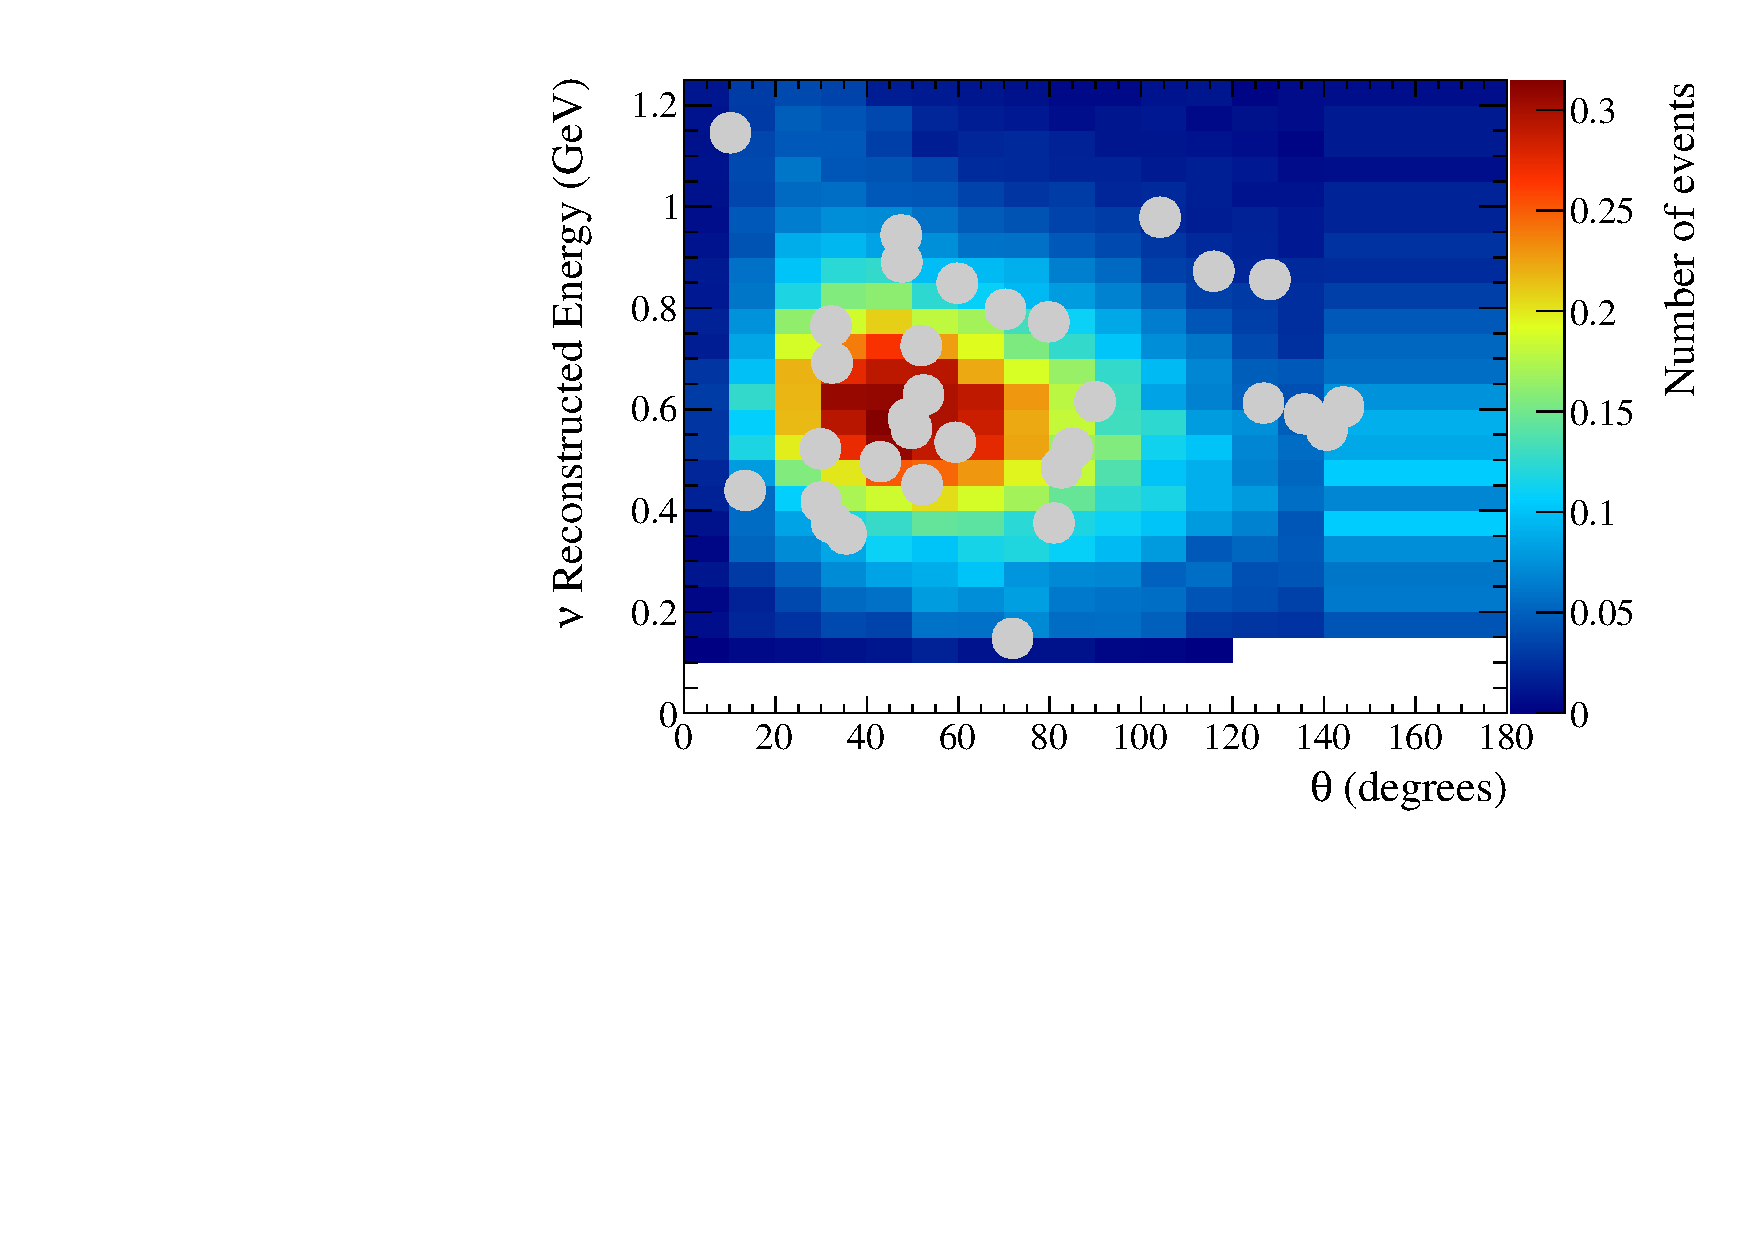
\includegraphics[width=0.9\textwidth]{./joint_plots/data/Run17b/spectrum_data_exp_1Re_Run17.pdf} 
\caption{Electron-like, neutrino mode}
\end{subfigure}
\begin{subfigure}[b]{0.49\textwidth}
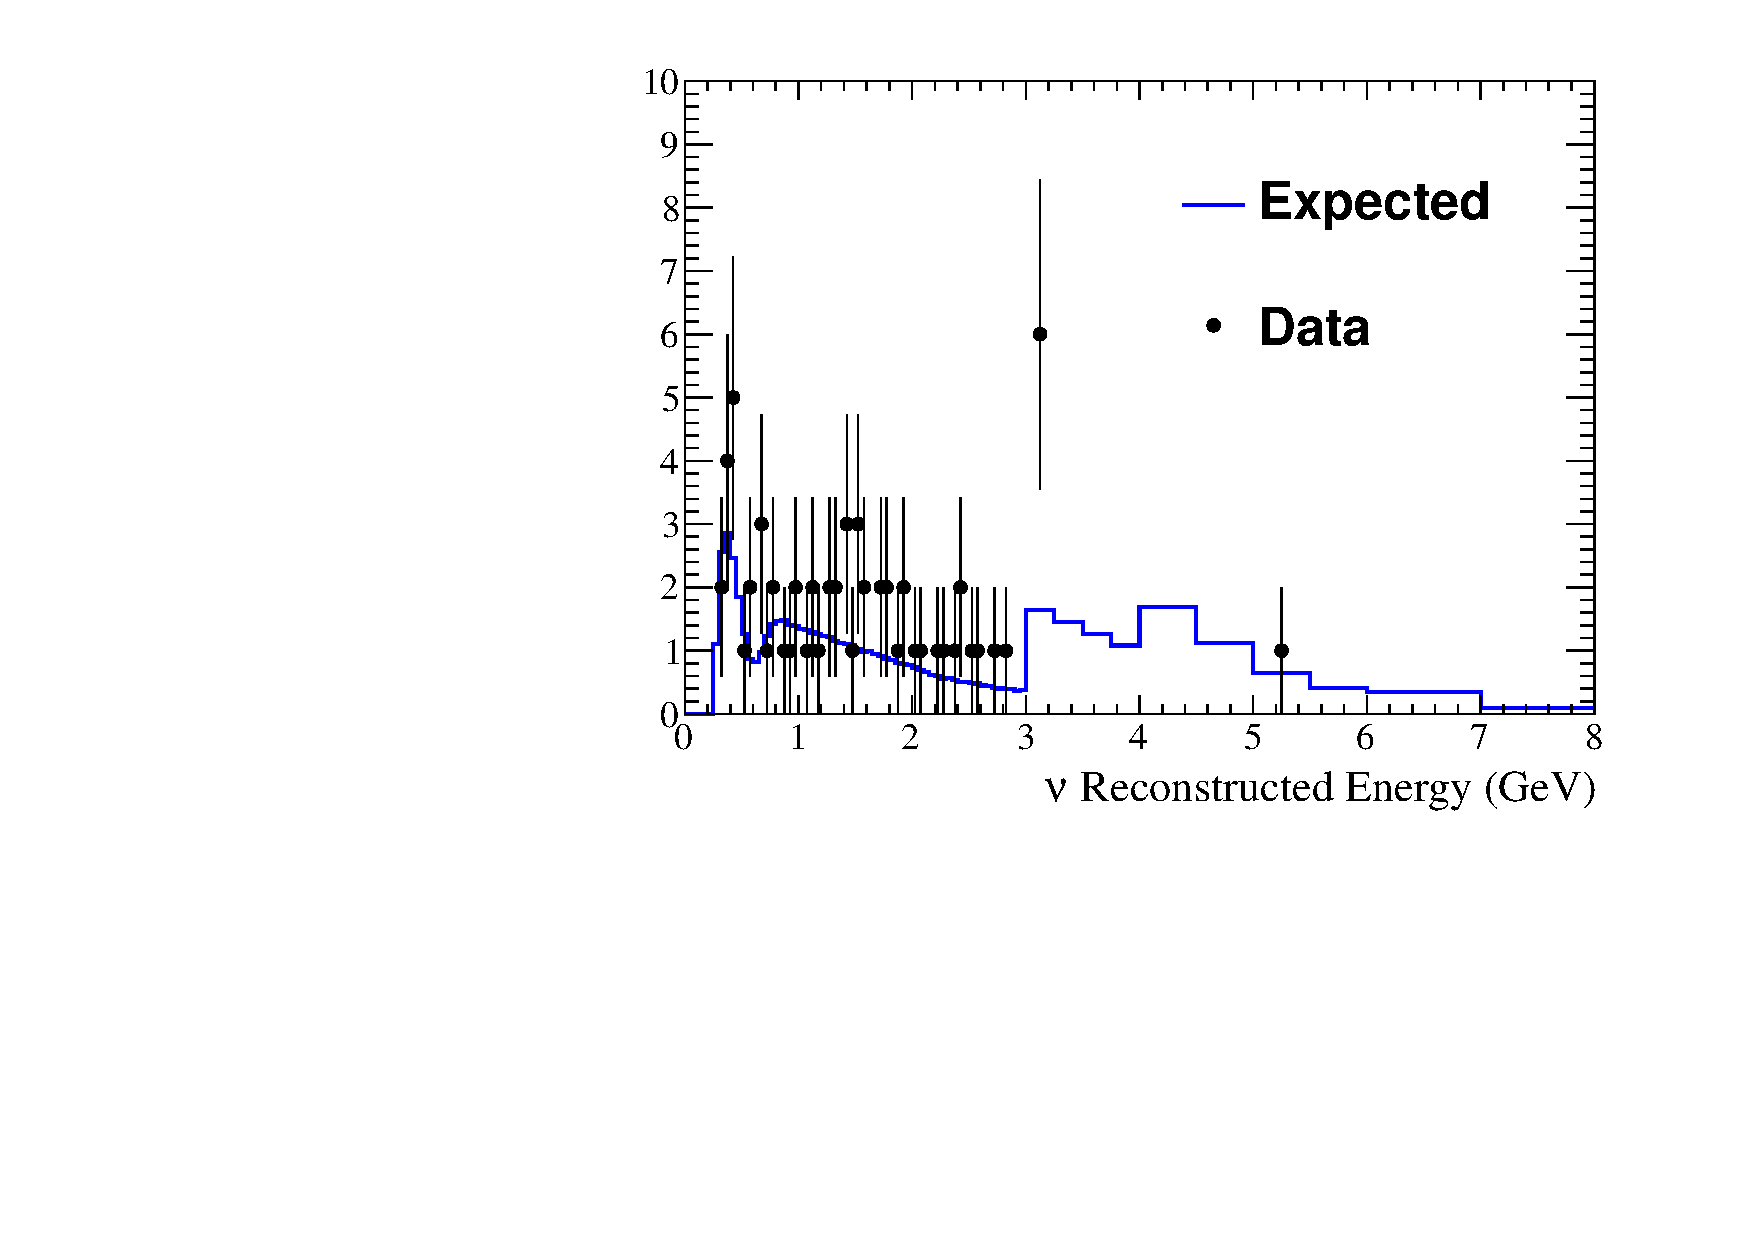
\includegraphics[width=0.9\textwidth]{./joint_plots/data/Run17b/spectrum_data_exp_RHC1Rmu_Run17.pdf} 
\caption{Muon-like, antineutrino mode}
\end{subfigure}
\begin{subfigure}[b]{0.49\textwidth}
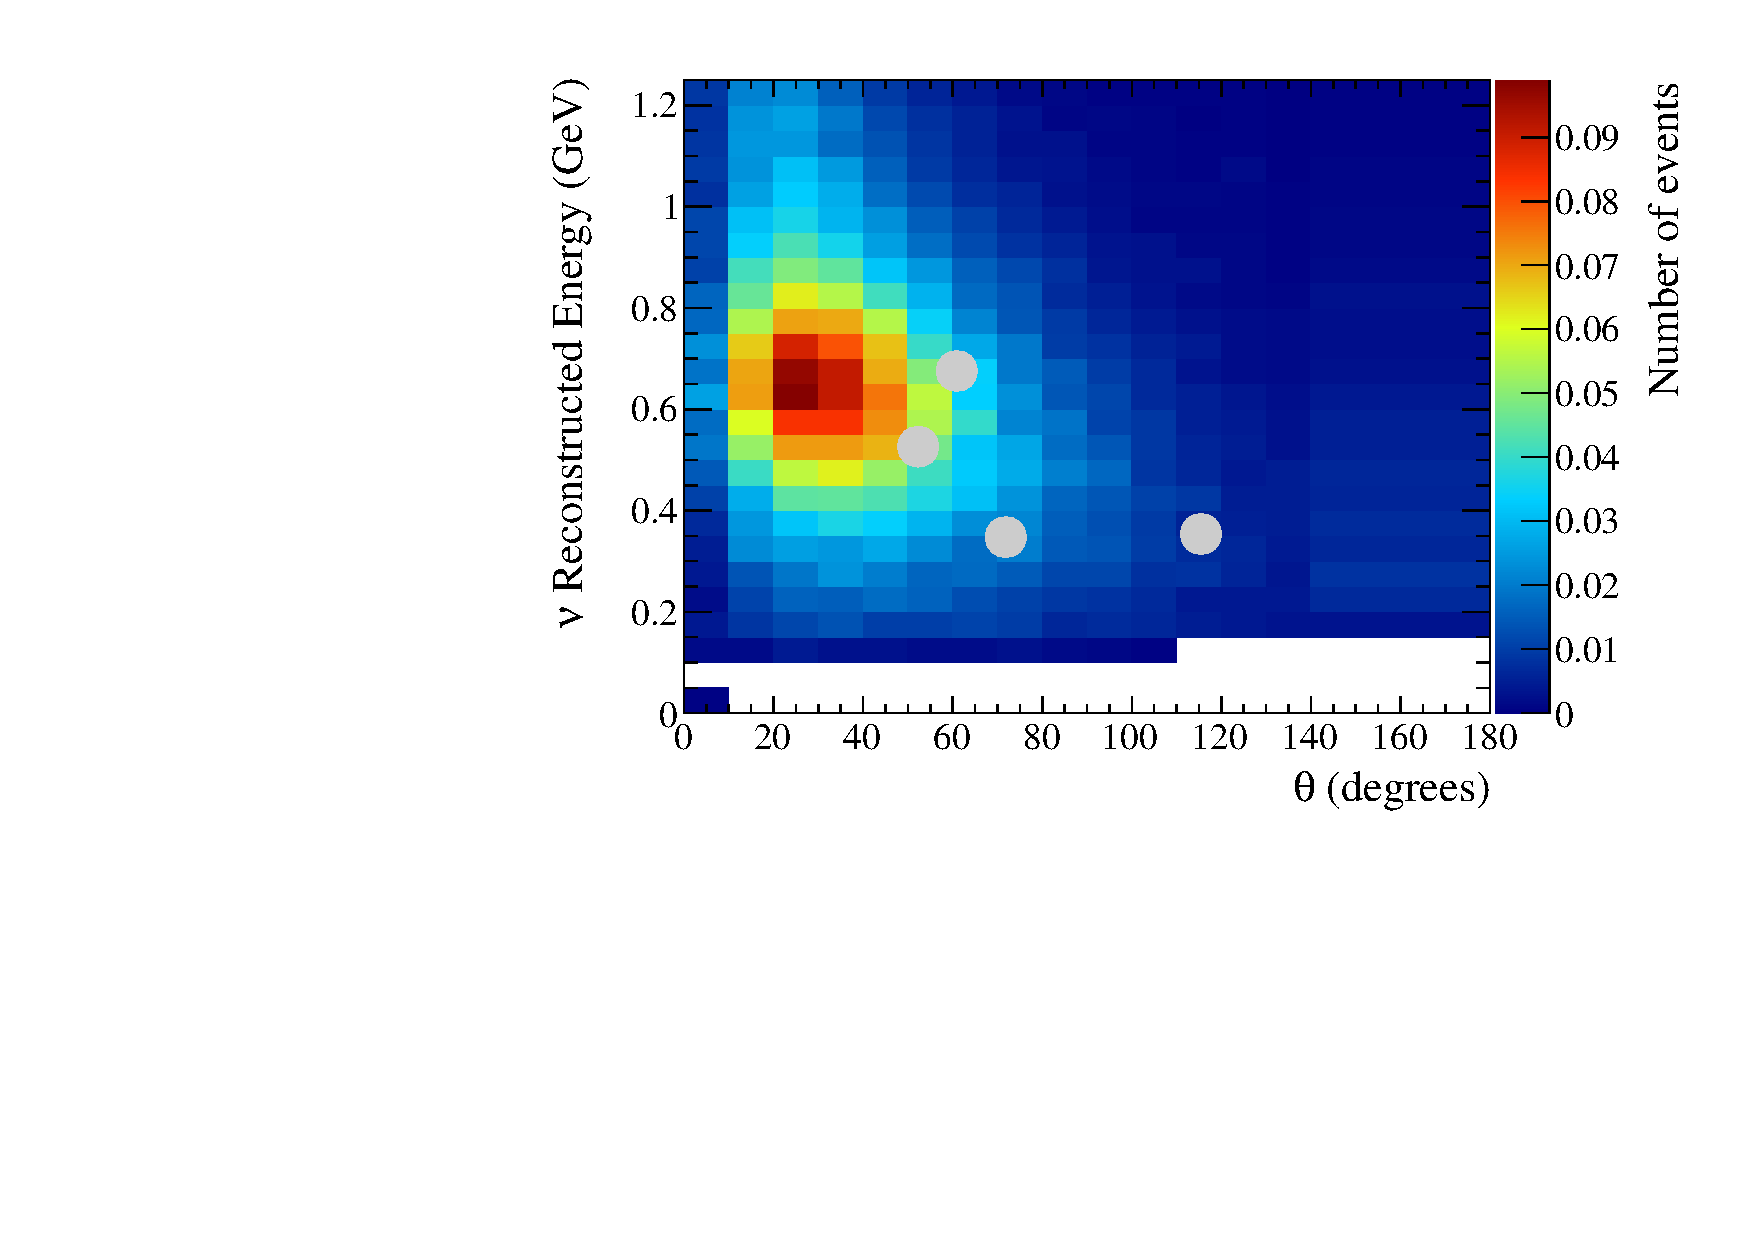
\includegraphics[width=0.9\textwidth]{./joint_plots/data/Run17b/spectrum_data_exp_RHC1Re_Run17.pdf} 
\caption{Electron-like, antineutrino mode}
\end{subfigure}
\caption {
The predicted spectra compared to the Run 1-7b dataset (dots),
which corresponds to an exposure 
of \TotalPotNuRunOneSevenB POT in neutrino mode
and
of \TotalPotNuBarRunOneSevenB POT in antineutrino mode,
are shown.
The expected distribution corresponds to the oscillation parameters of the Asimov data set A shown in \cref{tab:osc_params_joint_asimov}.
The spectra were generated with the systematic parameters measured with the ND280 data 
shown in \cref{tab:banff_uncertainties_flux_fhc},~\ref{tab:banff_uncertainties_flux_rhc},
~\ref{tab:banff_uncertainties_xsec} 
and the nominal Super-K systematic parameters shown in \cref{tab:banff_uncertainties_skdetfsi}.
}
\label{fig:spectra_expVsdata_asimov_A_run17b}
\end{figure}


% Table summarizing the # of observed events in Run 1-6

\begin{table}[htb]
\centering
\begin{tabular}{| c | c | c | c | c | c | c | c |}
\hline
Beam mode	& Sample		& Exp. Asimov A  	& Exp. Asimov A	& Exp. Asimov B	& Exp. Not Osc			& Observed 	& Best fit\\
			& 			& 			  	& ($\delta_{CP}=0$)	& 				& 					& 		 	& (reactors) \\
\hline
neutrino	 	& $\mu$-like 	&127.516			& 127.181			& 132.125	 		& 489.894				& 125 		& 126.913 \\
neutrino 		& $e$-like  	& 26.932 			& 22.692			& 20.208			& 5.770				& 32 			& 27.261 \\
antineutrino 	& $\mu$-like 	& 64.205			& 64.059			& 65.597			& 184.837				& 66 			& 63.845 \\
antineutrino 	& $e$-like 	& 6.004			& 6.902			& 6.252			& 2.335				& 4 			& 6.136 \\
\hline
\end{tabular}
\caption{
The observed, expected and best-fit number of events in Run 1-7b data set
for an exposure
of \TotalPotNuRunOneSevenB POT in neutrino mode
and
of \TotalPotNuBarRunOneSevenB POT in antineutrino mode
are shown 
for each selected sample.
The prediction is produced using the BANFF tuning
and the oscillation parameters shown in \cref{tab:osc_params_joint_asimov}.
The total number of events of the best-fit spectra is obtained by using \cref{eq:bestfit_spectrum_marg}.
}
\label{tab:num_events_run17b}
\end{table}













%--------------------------------------------------------------------------------------
%
% 1-dimensional chisq & best-fit
%
%--------------------------------------------------------------------------------------

\subsection {1-dimensional $\chi^2$ distributions and best-fit}
\label{sec:chisq_1d_run17b}


% 1-dimensional contours

1-dimensional $\chi^2$ distributions as in \cref{sec:sensi} are produced
and shown in \cref{fig:joint_data_fit_1d_run17b}.
The best-fit value of $\delta_{CP}$ when the reactor constraint is applied is -1.759
similar to the Run 1-6 one, i.e. -1.854 (see \cref{tab:joint_bestfit}), but closer to $-\pi/2$ (i.e. -1.571).
 
Looking at the $\chi^2$ distribution of $\sin^2 \theta_{13}$ with T2K only data in \cref{fig:joint_data_fit_1d}
we can see that the reactor measurements are 
in better agreement with the Run 1-7b data than the Run 1-6 ones (see \cref{fig:joint_data_fit_1d}).

\begin{figure*}[htb]
\center
\begin{subfigure}[b]{0.49\textwidth}
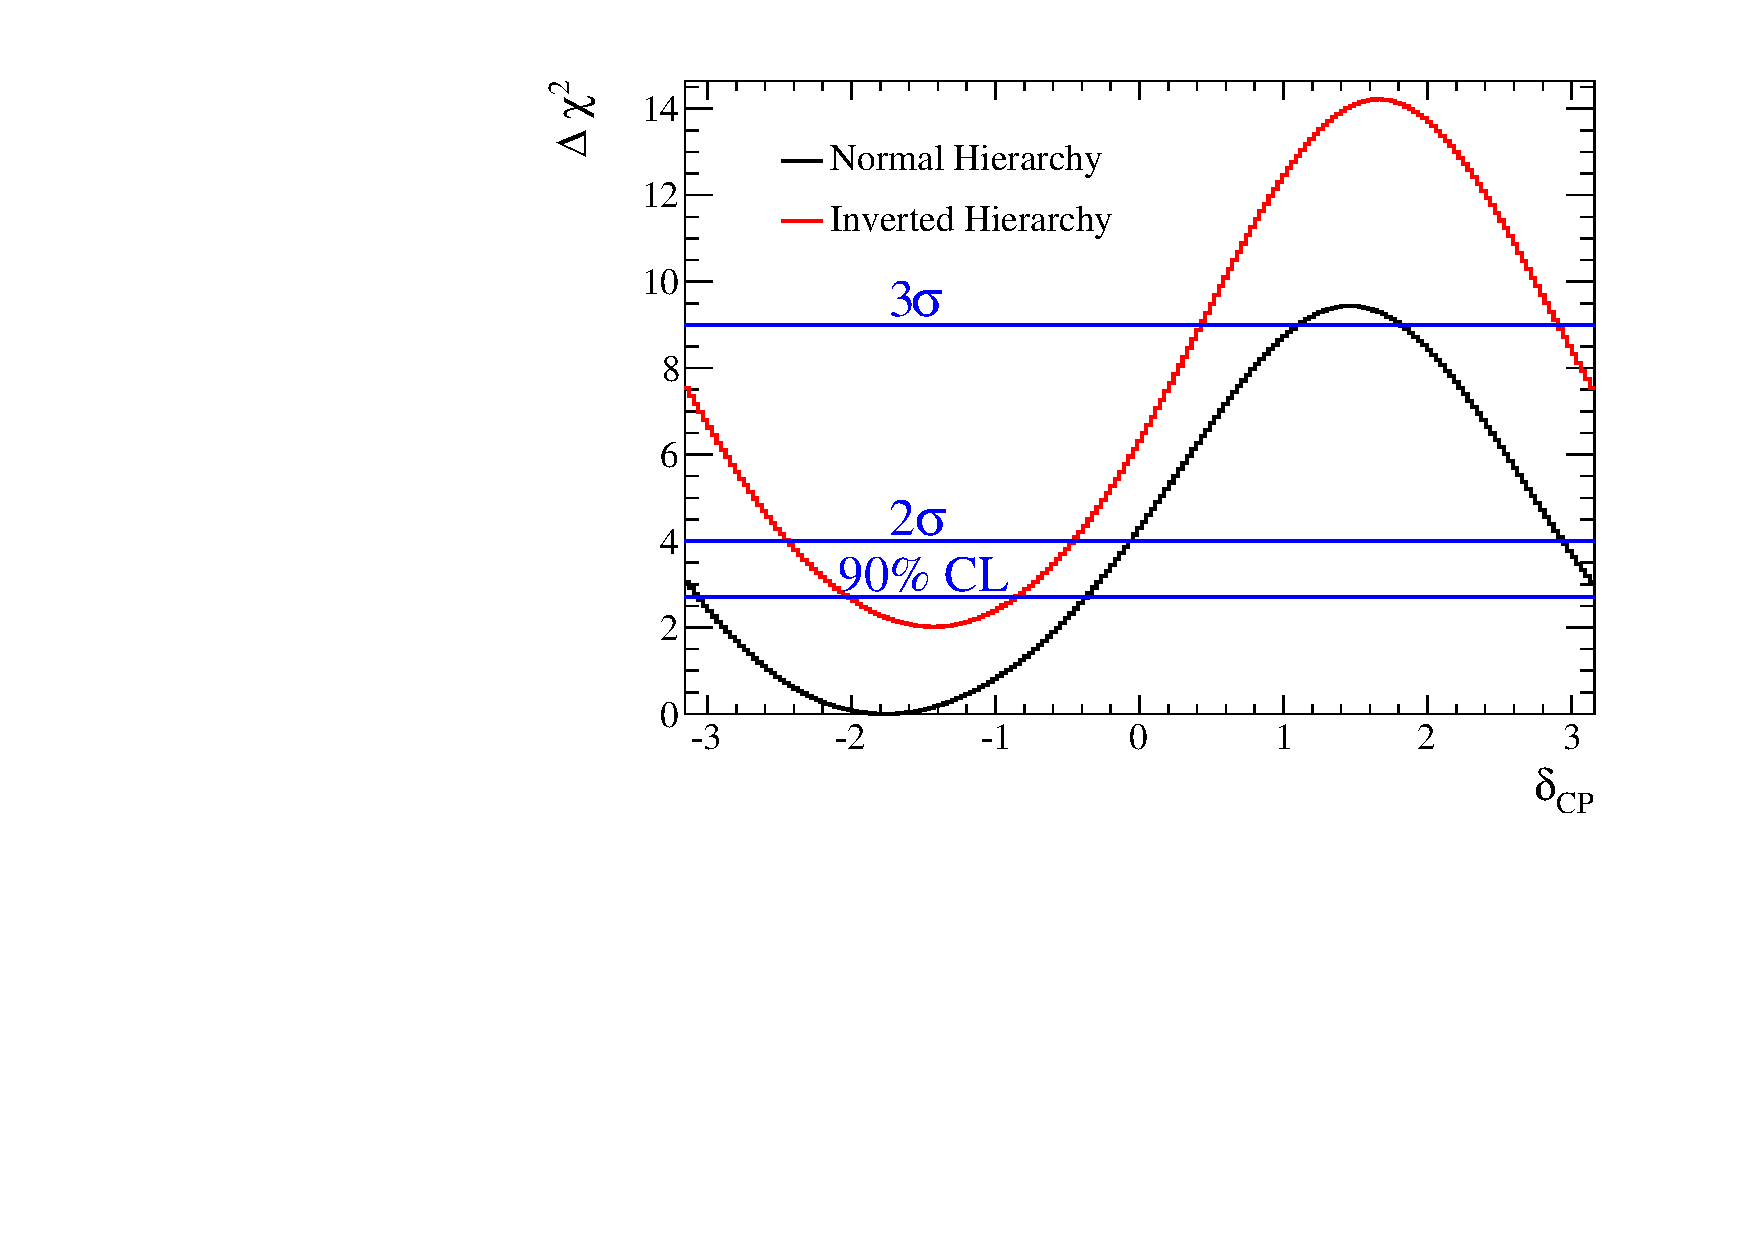
\includegraphics[width=0.9\textwidth]{joint_plots/data_contours/Run17b/dcp_react_data_run17_constdchisq.pdf}
\caption{$\delta_{CP}$ with reactor constraint}
\label{fig:dcp_fit_with_reactor_data}
\end{subfigure}
\begin{subfigure}[b]{0.49\textwidth}
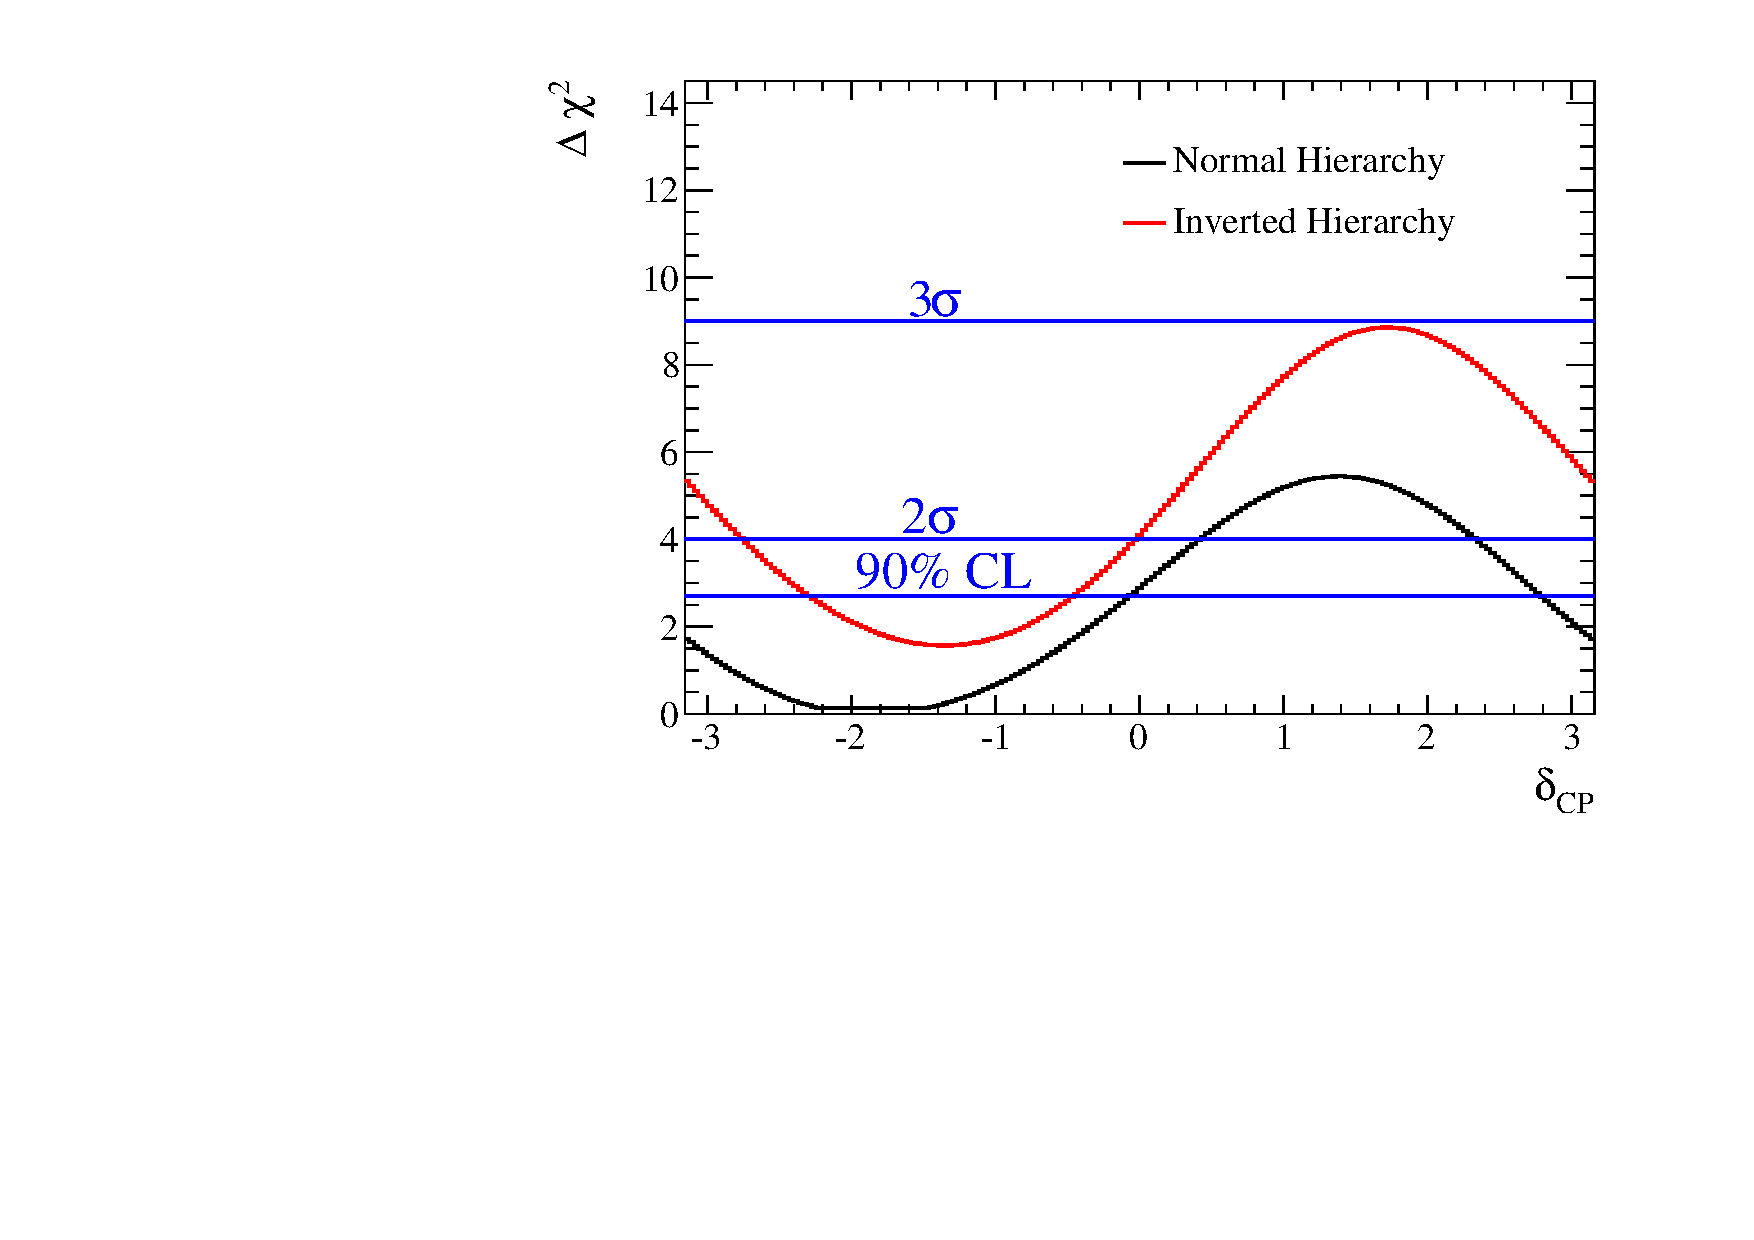
\includegraphics[width=0.9\textwidth]{joint_plots/data_contours/Run17b/dcp_t2konly_data_run17_constdchisq.pdf}
\caption{$\delta_{CP}$ with T2K data only}
\end{subfigure}
\begin{subfigure}[b]{0.49\textwidth}
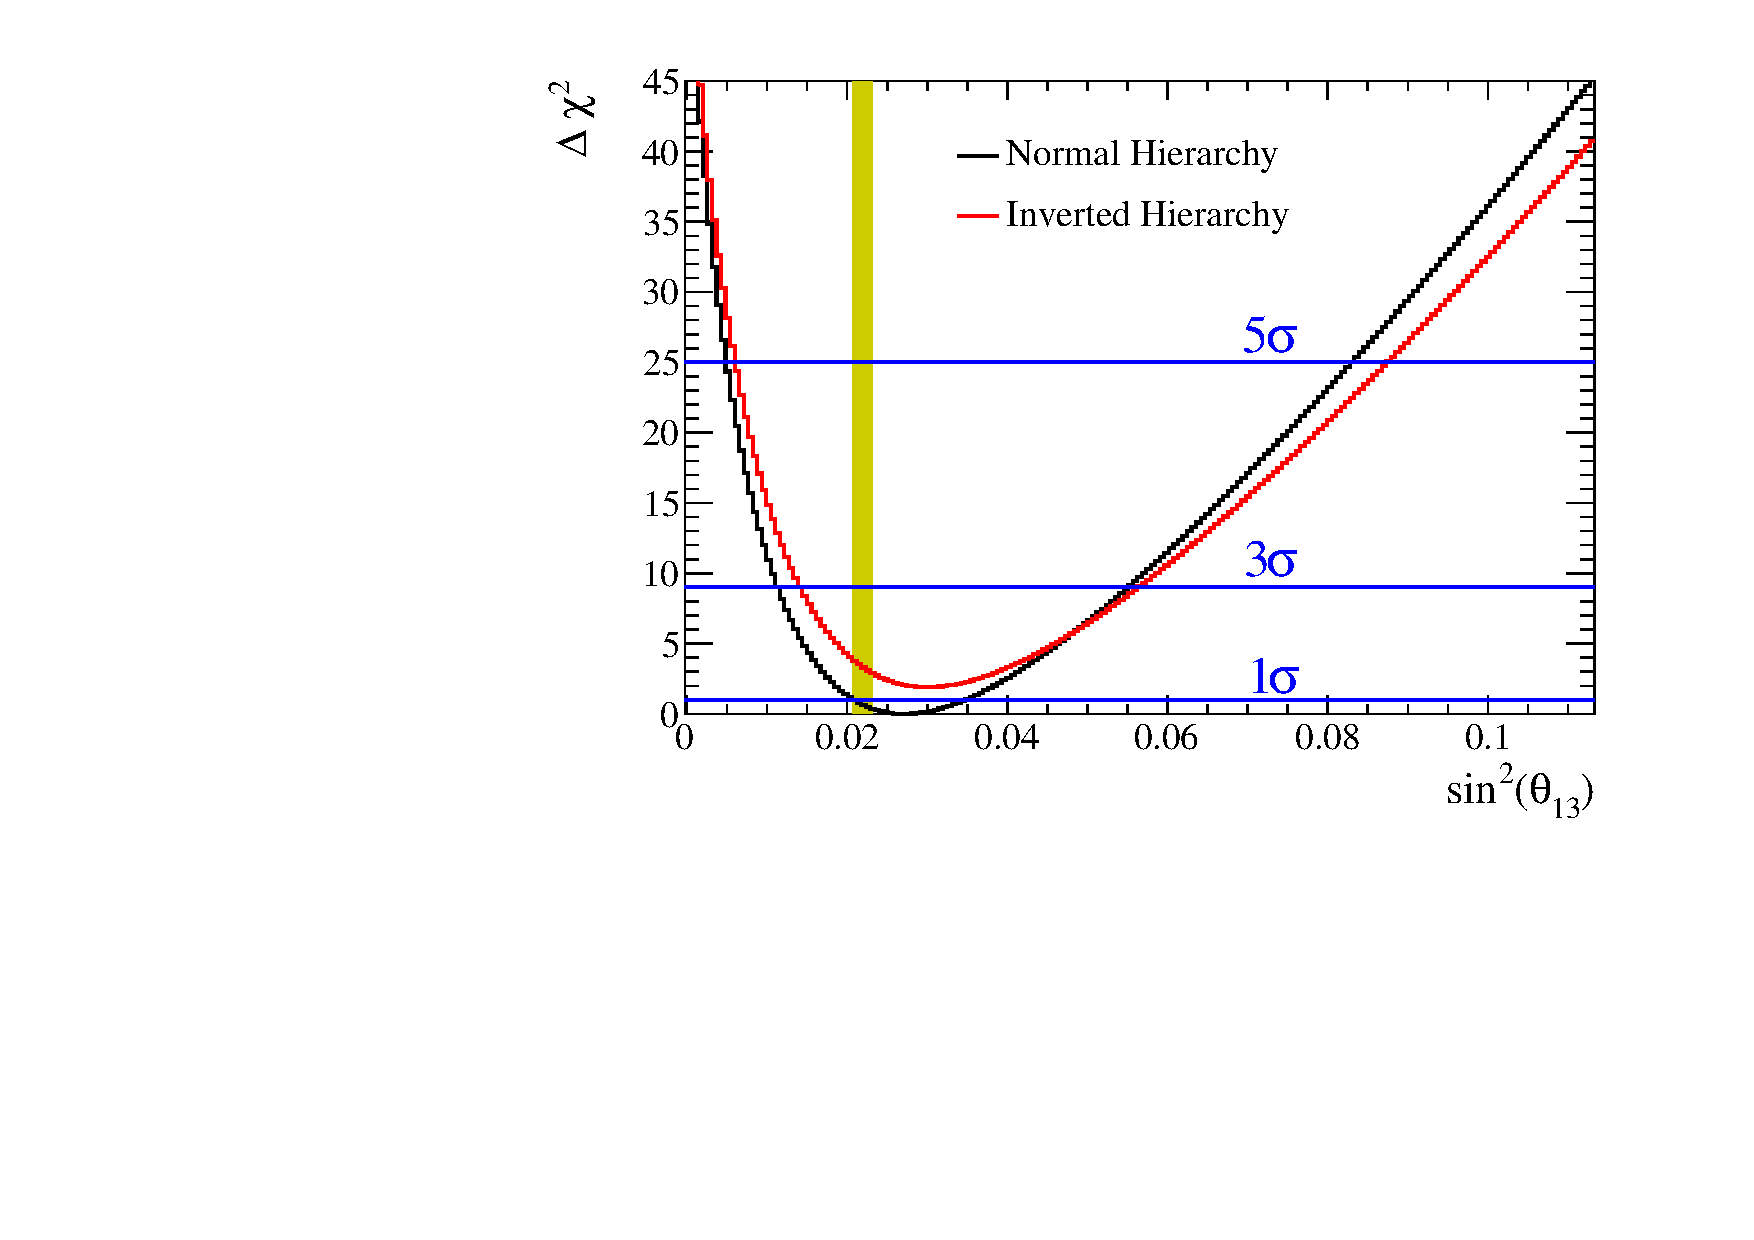
\includegraphics[width=0.9\textwidth]{joint_plots/data_contours/Run17b/sinsqth13_t2konly_data_run17_constdchisq.pdf}
\caption{$\sin^2 \theta_{13}$ with T2K data only}
\end{subfigure}
\begin{subfigure}[b]{0.49\textwidth}
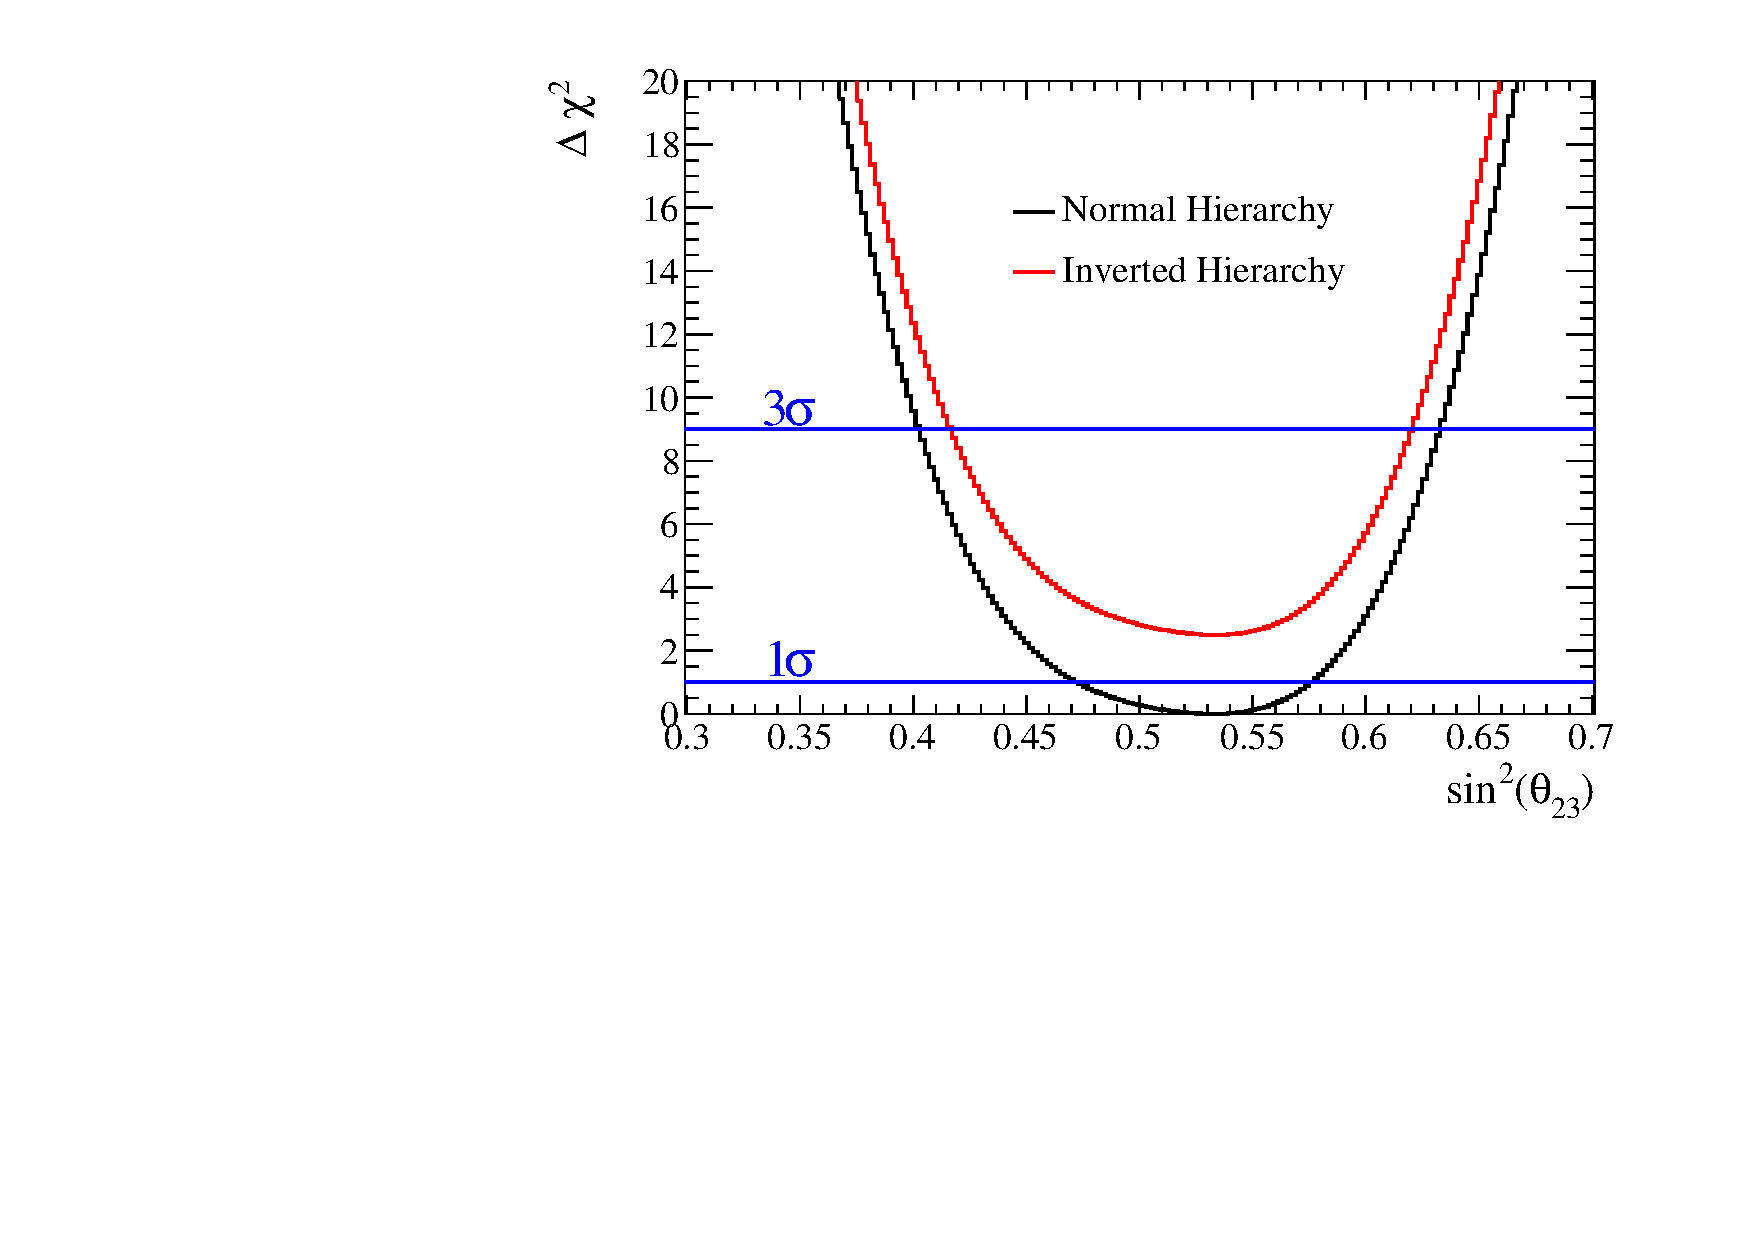
\includegraphics[width=0.9\textwidth]{joint_plots/data_contours/Run17b/sinsqth23_react_data_run17_constdchisq.pdf}
\caption{$\sin^2 \theta_{23}$ with reactor constraint}
\end{subfigure}
\begin{subfigure}[b]{0.49\textwidth}
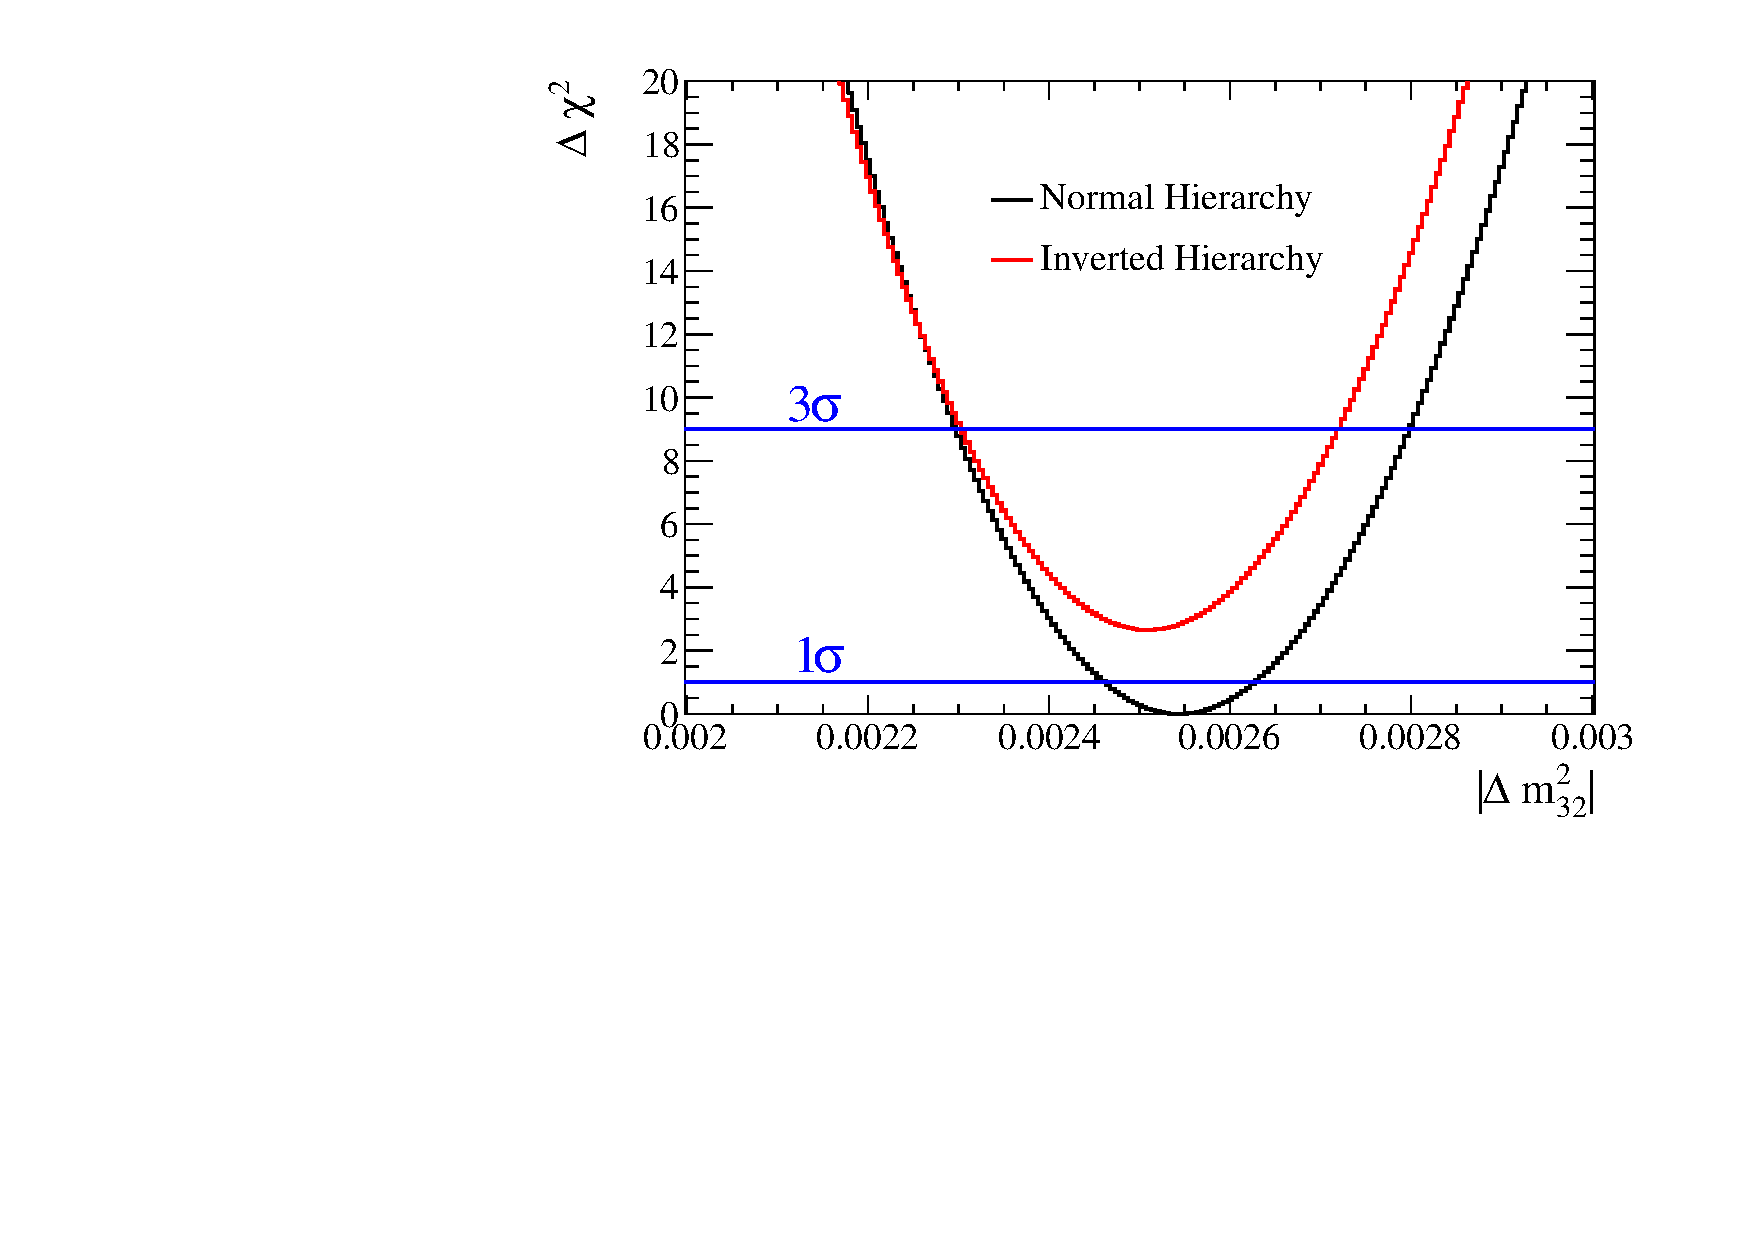
\includegraphics[width=0.9\textwidth]{joint_plots/data_contours/Run17b/dmsq_react_data_run17_constdchisq.pdf}
\caption{$\Delta m^2_{32}$ ($\Delta m^2_{13}$) with reactor constraint}
\end{subfigure}
\caption{
Measured $\Delta \chi^2$ distributions
with the full Run 1-7b data set.
Both normal (black) and inverted (red) hierarchies are shown. 
The \emph{constant} $\Delta \chi^2$ method is used. %(see \cref{app:method_cl}).
Both normal and inverted hierarchy $\Delta \chi^2$ distributions are shifted with respect to the same global minimum. 
All the oscillation parameters which are not parameters of interest
are marginalised using the prior distributions shown in \cref{tab:marg_binnning}.
The measured $\Delta \chi^2$ distribution as a function of $\sin^2 \theta_{13}$ is compared
with the value given by the global analysis of the reactor measurements,
$\sin^2 \theta_{13} = 0.0219 \pm 0.0012 $
\cite{pdg_2014},
shown by the yellow bar.
}
\label{fig:joint_data_fit_1d_run17b}
\end{figure*}

%
% Neutrino only Vs AntiNeutrino only
%
%In \cref{fig:joint_dcp_nu_nubar}
%the $\chi^2$ distributions as a function of $\delta_{CP}$
%with reactor constraint
%is obtained by 
%running the analysis using either only neutrino 
%or antineutrino mode samples for the Run 1-6 data set,
%in order to check the compatibility of neutrino and antineutrino mode data.
%The result is mainly driven by the excess of the observed number
%of events in $e$-like neutrino mode sample compared to what is expected.
%Though the significance given by the antineutrino mode samples is still low,
%also given by the fact that $\sin^2 \theta_{23}$ is not constrained 
%by the antineutrino mode $\mu$-like sample
%as much as by  
%the neutrino mode $\mu$-like sample,
%it is interesting to note that the antineutrino data also prefer 
%a value of $\delta_{CP}$ close to $-\pi / 2$.
%
%\begin{figure*}[htb]
%\center
%%
\includegraphics[width=0.9\textwidth]{./images/missing_plot-eps-converted-to.pdf}
%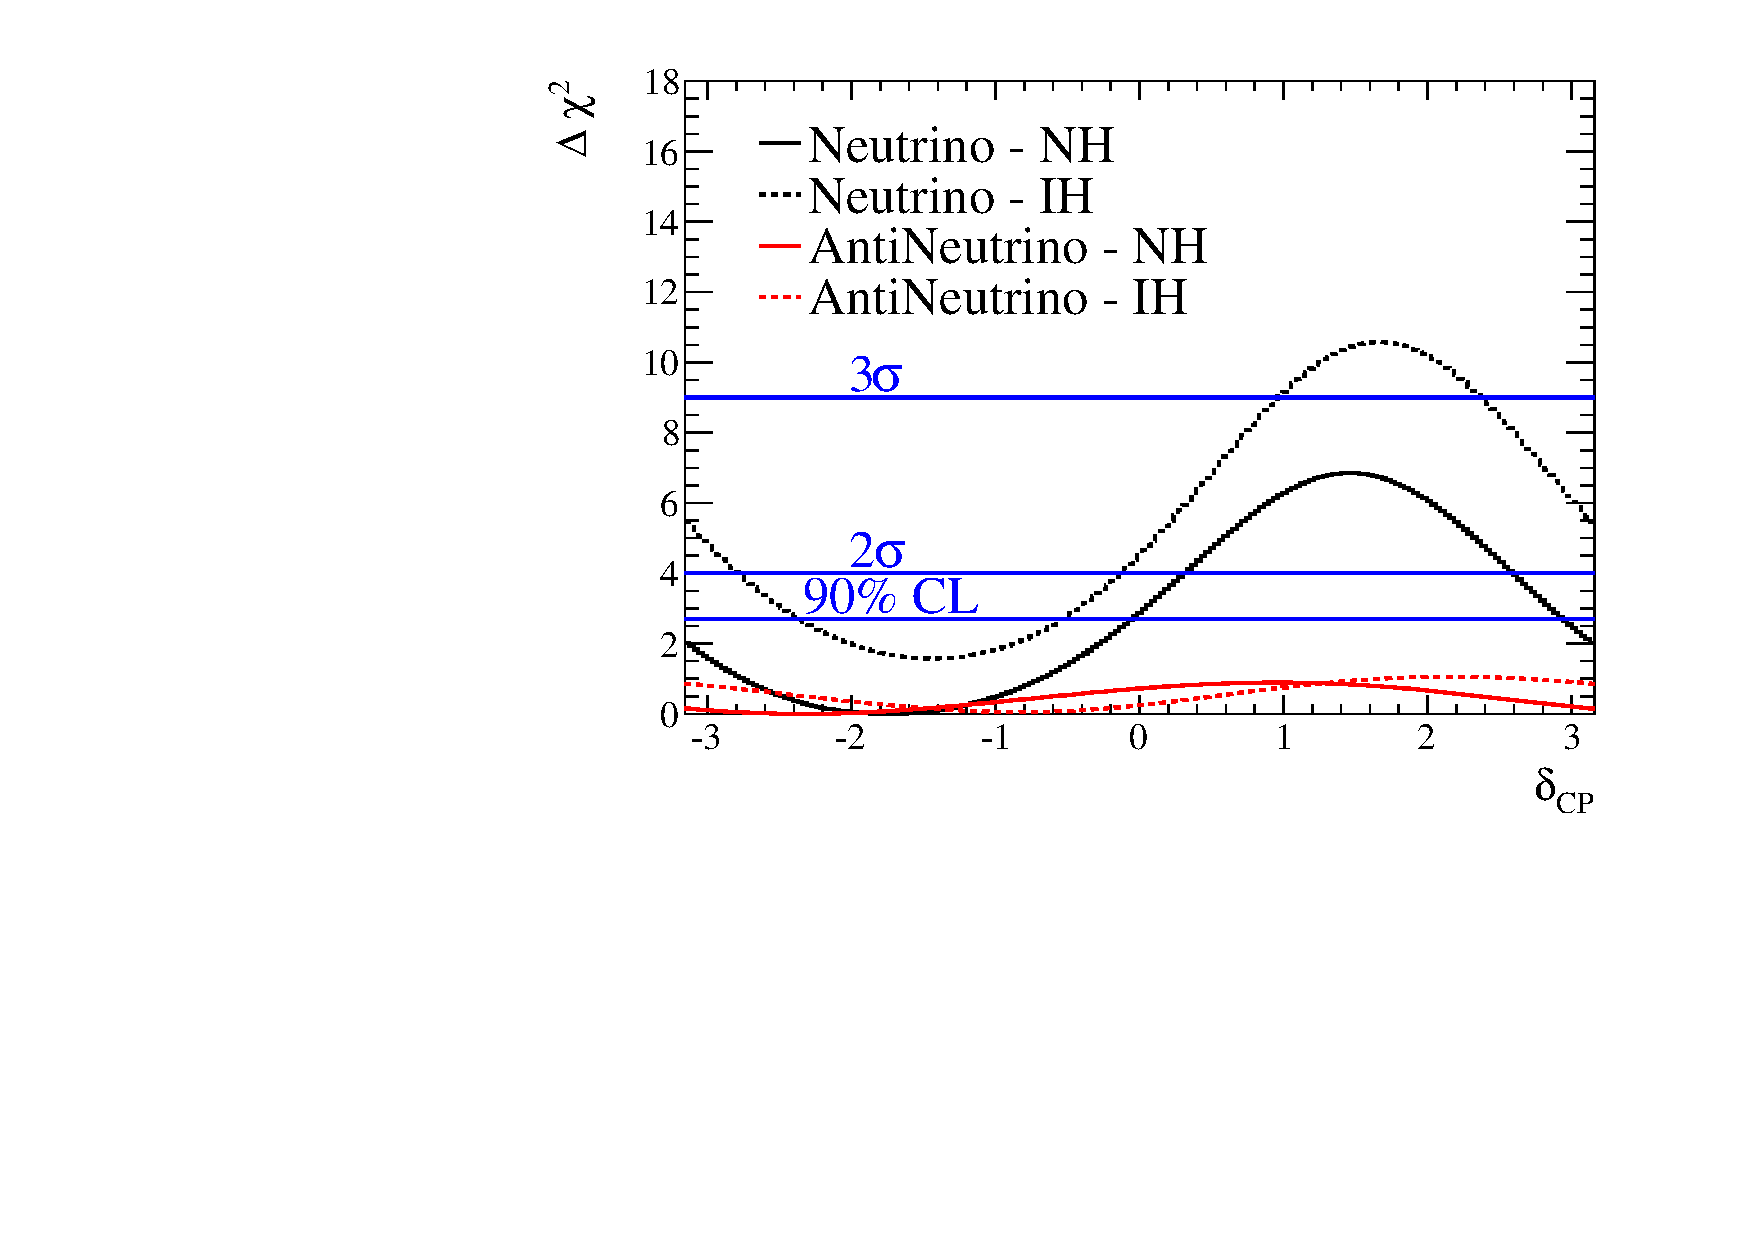
\includegraphics[width=0.5\textwidth]{./joint_plots/data_contours/dcp_react_data_constdchisq_fhcVsrhc.pdf}
%\caption{
%Measured $\Delta \chi^2$ distributions
%with the full Run 1-6 data set
%as a function of
%$\delta_{CP}$ 
%with reactor constraint
%independently for only neutrino and antineutrino mode data.
%Both normal (black) and inverted (red) hierarchies are shown. 
%%Both 68\% (dashed line) and 90\% CL (solid line) are shown.
%%For $\delta_{CP}$ confidence intervals are performed using the
%%\emph{Feldman-Cousins} method,
%%while for the other oscillation parameters
%The \emph{constant} $\Delta \chi^2$ method is used. %(see \cref{app:method_cl}).
%Both normal and inverted hierarchy $\Delta \chi^2$ distributions are shifted with respect to the same global minimum,
%independently for the neutrino and antineutrino mode data. 
%All the oscillation parameters which are not parameters of interest
%are marginalised using the prior distributions shown in \cref{tab:marg_binnning}.
%}
%\label{fig:joint_dcp_nu_nubar}
%\end{figure*}


%
% Rate-only analysis
%
%In \cref{fig:joint_data_fit_1d_rateonly} the $\chi^2$ distributions as a function of $\delta_{CP}$
%is obtained by performing a rate-only analysis; 
%instead of using the shape information of the $E_{reco}$ vs $\theta_l$ spectra,
%the total number of events of each sample is fitted, 
%reducing the $E_{reco}$ vs $\theta_l$ template to 1 bin.
%Then the best-fit value of $\delta_{CP}$ is -1.602 closer to $-\pi/2$ with respect to the case
%where the shape information is used.
%
%\begin{figure*}[htb]
%\center
%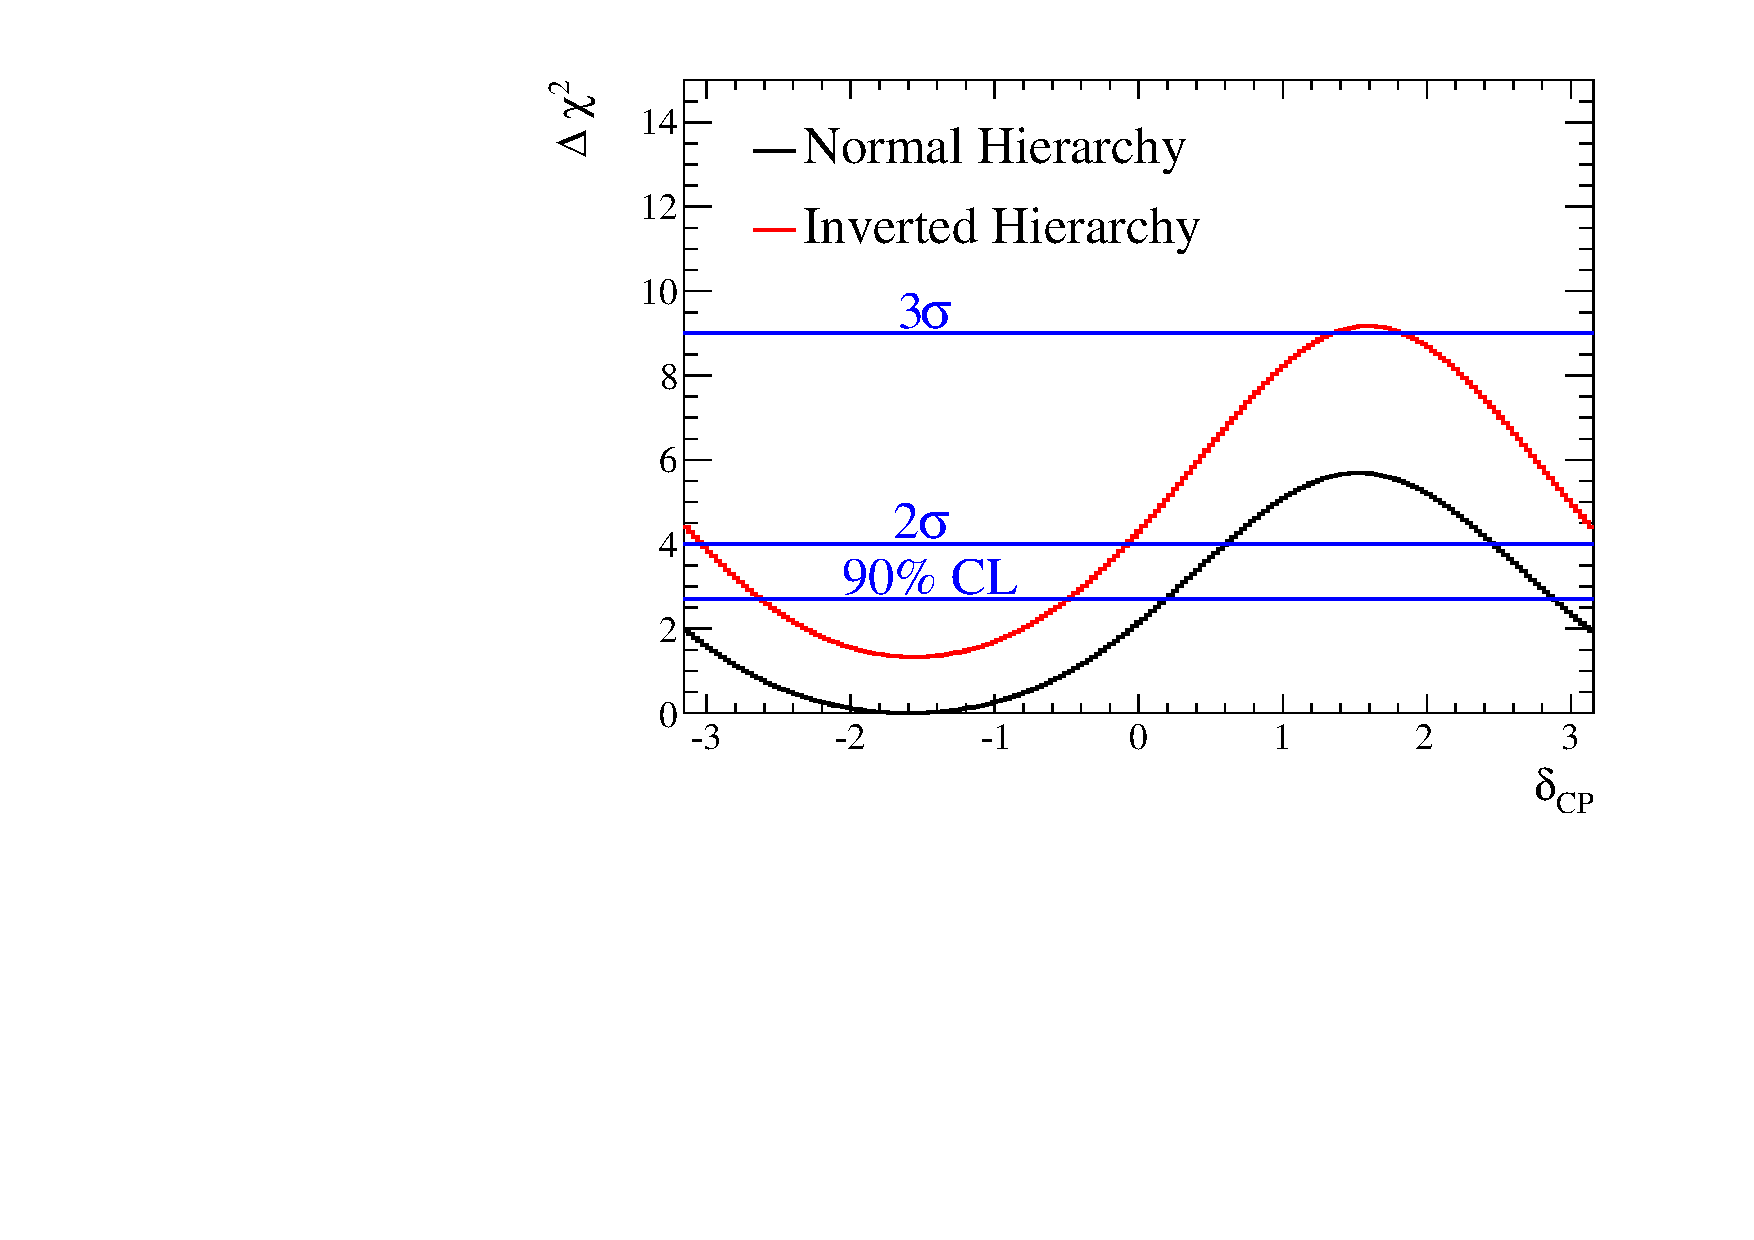
\includegraphics[width=0.5\textwidth]{joint_plots/data_contours/dcp_react_data_constdchisq_rateonly.pdf}
%\caption{
%Measured $\Delta \chi^2$ distributions
%with a rate-only analysis
%using the full Run 1-6 data set
%as a function of
%$\delta_{CP}$ 
%with reactor constraint.
%Both normal (black) and inverted (red) hierarchies are shown. 
%%Both 68\% (dashed line) and 90\% CL (solid line) are shown.
%%For $\delta_{CP}$ confidence intervals are performed using the
%The \emph{constant} $\Delta \chi^2$ method is used. %(see \cref{app:method_cl}).
%Both normal and inverted hierarchy $\Delta \chi^2$ distributions are shifted with respect to the same global minimum. 
%All the oscillation parameters which are not parameters of interest
%are marginalised using the prior distributions shown in \cref{tab:marg_binnning}.
%}
%\label{fig:joint_data_fit_1d_rateonly}
%\end{figure*}




% Table of best-fit and 1sigma ranges

In \cref{tab:joint_bestfit_run17b} the best-fit values as well as the $1\sigma$ ranges for each 
oscillation parameter are shown for the Run 1-7b data fit, for both normal and inverted hierarchy.
The $1\sigma$ ranges are extracted for each oscillation parameter
from the 1-dimensional $\Delta \chi^2$ distributions shown in \cref{fig:joint_data_fit_1d_run17b},
where one oscillation parameter is free and all the other oscillation as well as the systematic 
parameters are marginalised.
The mass hierarchy is minimized:
for both normal and inverted hierarchy the $1\sigma$ ranges are calculated with respect to the 
same global minimum.
Since this approach is not entirely correct and there does not exist any procedure 
to set more reliable confidence intervals which does not consist of toy MC studies (see \cref{sec:cl_mh}),
the advice to the reader is to give more importance to the difference in $\chi^2_{marg}$
between normal and inverted hierarchies in the respective best-fit points, 
instead of the $1\sigma$ ranges of inverted hierarchy, 
which are smaller by construction.
It is also worth to notice that the $1\sigma$ ranges for normal hierarchy (best-fit)
are set correctly with the constant $\Delta \chi^2$ method in the gaussian approximation.

As already written above, the Run 1-7b best-fit value of $\delta_{CP}$ with reactor constraint is 
close to the Run 1-6 one (see \cref{tab:joint_bestfit}).
However if the reactor constraint is not applied, the Run 1-7b best-fit value of $\delta_{CP}$
is quite different with respect to the Run 1-6 one:
the best-fit for both normal and inverted hierarchy gets closer to $-\pi/2$.
Indeed, as shown in \cref{fig:joint_data_fit_1d_run17b}, 
the $\Delta \chi^2$ distribution as a function of $\delta_{CP}$ and mass hierarchy
with T2K only data becomes more similar to the one obtained with the reactor constraint:
assuming the constant $\Delta \chi^2$ method, $\delta_{CP}=0$ for normal hierarchy
is excluded at 90\%CL and the maximal $\Delta \chi^2$ value is 
larger than 4.5 and 8.5 respectively for normal and inverted hierarchy.
The exclusion is stronger than the one given by the Run 1-6 where
almost the full range $\delta_{CP}$ and normal hierarchy was allowed at 90\%CL.
This is due to the downward fluctuation in the antineutrino mode $e$-like sample
combined with an upward fluctuation in the neutrino mode $e$-like sample.
Assuming Asimov data set A but with $\delta_{CP} = 0$ we expect 6.9
antineutrino mode $e$-like events and 22.7 neutrino mode $e$-like events.
If we assume $\delta_{CP}=-1.601$ we expect 26.9 and 6.0 events 
for neutrino and antineutrino mode $e$-like samples.
However we observe only 4 events in antineutrino mode and 
32 events in neutrino mode $e$-like samples.
Consequently the Run 1-7b data favor a smaller value of $\sin^2 \theta_{13}$,
in better agreement with the reactor measurement,
enhancing the tension due to the excess in the neutrino mode $e$-like sample.

It is interesting to notice that the Run 1-7b $\pm 1\sigma$ interval of $\sin^2 \theta_{23}$ is slightly larger
than the Run 1-6 one though the number of events in antineutrino mode $\mu$-like samples is almost double. 
This can be qualitatively understood by comparing the observed and expected number of events
in \cref{tab:num_events_run17b} (Run 1-7b) and~\ref{tab:num_events} (Run 1-6).
In Run 1-6 data set the observed number of $\bar{\nu}_{\mu}$ candidates is 34, in good agreement
with Asimov data set A, i.e. maximal disappearance, while in Run 1-7b data set we observe 66 events
which is closer to the Asimov data set B, i.e. lower octant ($\sin^2 \theta_{23} = 0.45$).


\begin{table}[htb]
\centering
\begin{tabular}{| c | c || c | c | c || c | c | c |}
\hline
								& {\bf Reactors}		& \multicolumn{3}{c||}{\bf Normal Hierarchy} & \multicolumn{3}{c|}{\bf Inverted Hierarchy} \\
\hline										
\bf Parameter						&				& Best-fit	& $\chi^2_{min}$	& $\pm 1\sigma$ 	  	 	& Best-fit		& $\chi^2_{min}$ 	& $\pm 1\sigma$ global (inverted) 	 \\
\hline
$\delta_{CP}$             				& YES      			& -1.759  	& 325.94			& [-2.569; -0.916]			& -1.445		& 327.96			& -							\\
								& 				& 		& 				& 						& 			& 				& ([-2.148; -0.737])				\\ 
\hline
$\delta_{CP}$            				& NO        			& -1.854  	& 329.10			& [-2.832;-0.802]  			& -1.351		& 330.67			& -				\\
								& 				& 		& 				& 						& 			& 				& ([-2.235; -0.514]) 				\\ 
\hline
$\sin^2 \theta_{13}$    				& NO             		& 0.0271  	& 327.20			& [0.0208; 0.0347]	        		& 0.0299		& 329.11			& -							\\
								& 				& 		& 				& 						& 			& 				& ([0.0231; 0.0384]) 				\\ 
\hline
$\sin^2 \theta_{23}$                      		& YES       		& 0.532	& 325.61			& [0.472; 0.576]			& 0.534		& 328.11			& -                 					\\
								& 				& 		& 				& 						& 			& 				& ([0.475; 0.575])			  	\\ 
\hline
$\Delta m^2_{32}$ or $\Delta m^2_{13}$   & YES  			& 2.545 	& 324.85 			& [2.461; 2.627]			& 2.510 		& 327.51			& -     						\\
($10^{-3} ~\text{eV}^2 / c^4$) 			& 				& 		&				&						&			&				& ([2.427; 2.592])				\\

\hline
\end{tabular}
\caption{
The Run 1-7b measured oscillation parameter best-fit
and minimum $\chi^2$ 
values  
as well as the 
$1\sigma$ 
CL intervals are shown,
for both normal and inverted hierarchy. 
The $\pm1\sigma$ interval is obtained by using the 
\emph{constant} $\Delta \chi^2$ method.
All the parameters are measured using the reactor constraint 
$\sin^2 2\theta_{13} = 0.085 \pm 0.005 $
\cite{pdg_2014},
except for $\delta_{CP}$ and $\sin^2 \theta_{13}$.
For the inverted hierarchy the intervals are calculated both with respect to 
the global minimum, i.e. normal hierarchy, as well as 
independently for inverted hierarchy (between parenthesis in second row).
As explained in \cref{sec:cl_mh}, the gaussian approximation does not work well 
for discrete parameters like the mass hierarchy however, since there is not a clear way
to compute $1\sigma$ ranges for both mass hierarchies without performing
CPU intensive toy MC studies, the constant $\Delta \chi^2$ method is used.
}                                                                                                                                                                                          
\label{tab:joint_bestfit_run17b}
\end{table}







% Best-fit spectra

The best-fit spectra, shown in \cref{fig:joint_spectra_bf_run17b} are computed as described in \cref{sec:spectra_bestfit_method}
and are compared to the unoscillated nominal spectra.
For $e$-like samples, where 2-dimensional templates are used,
the projection onto the reconstructed neutrino energy axis is shown.
All the systematic and oscillation parameters are marginalised following the procedure described in \cref{sec:spectra_bestfit_method},
while $\sin^2\theta_{23}$, $\delta_{CP}$ and the mass hierarchy were fixed to their best-fit values 
obtained from their simultaneous fit, i.e. \cref{fig:ss23_dcp_with_reactor_data_fit_run17b}.
Indeed these oscillation parameters have the strongest effect on the measurement,
since $\sin^2\theta_{13}$ is constrained with the reactor measurement.

\begin{figure*}[htb]
\center
\begin{subfigure}[b]{0.49\textwidth}
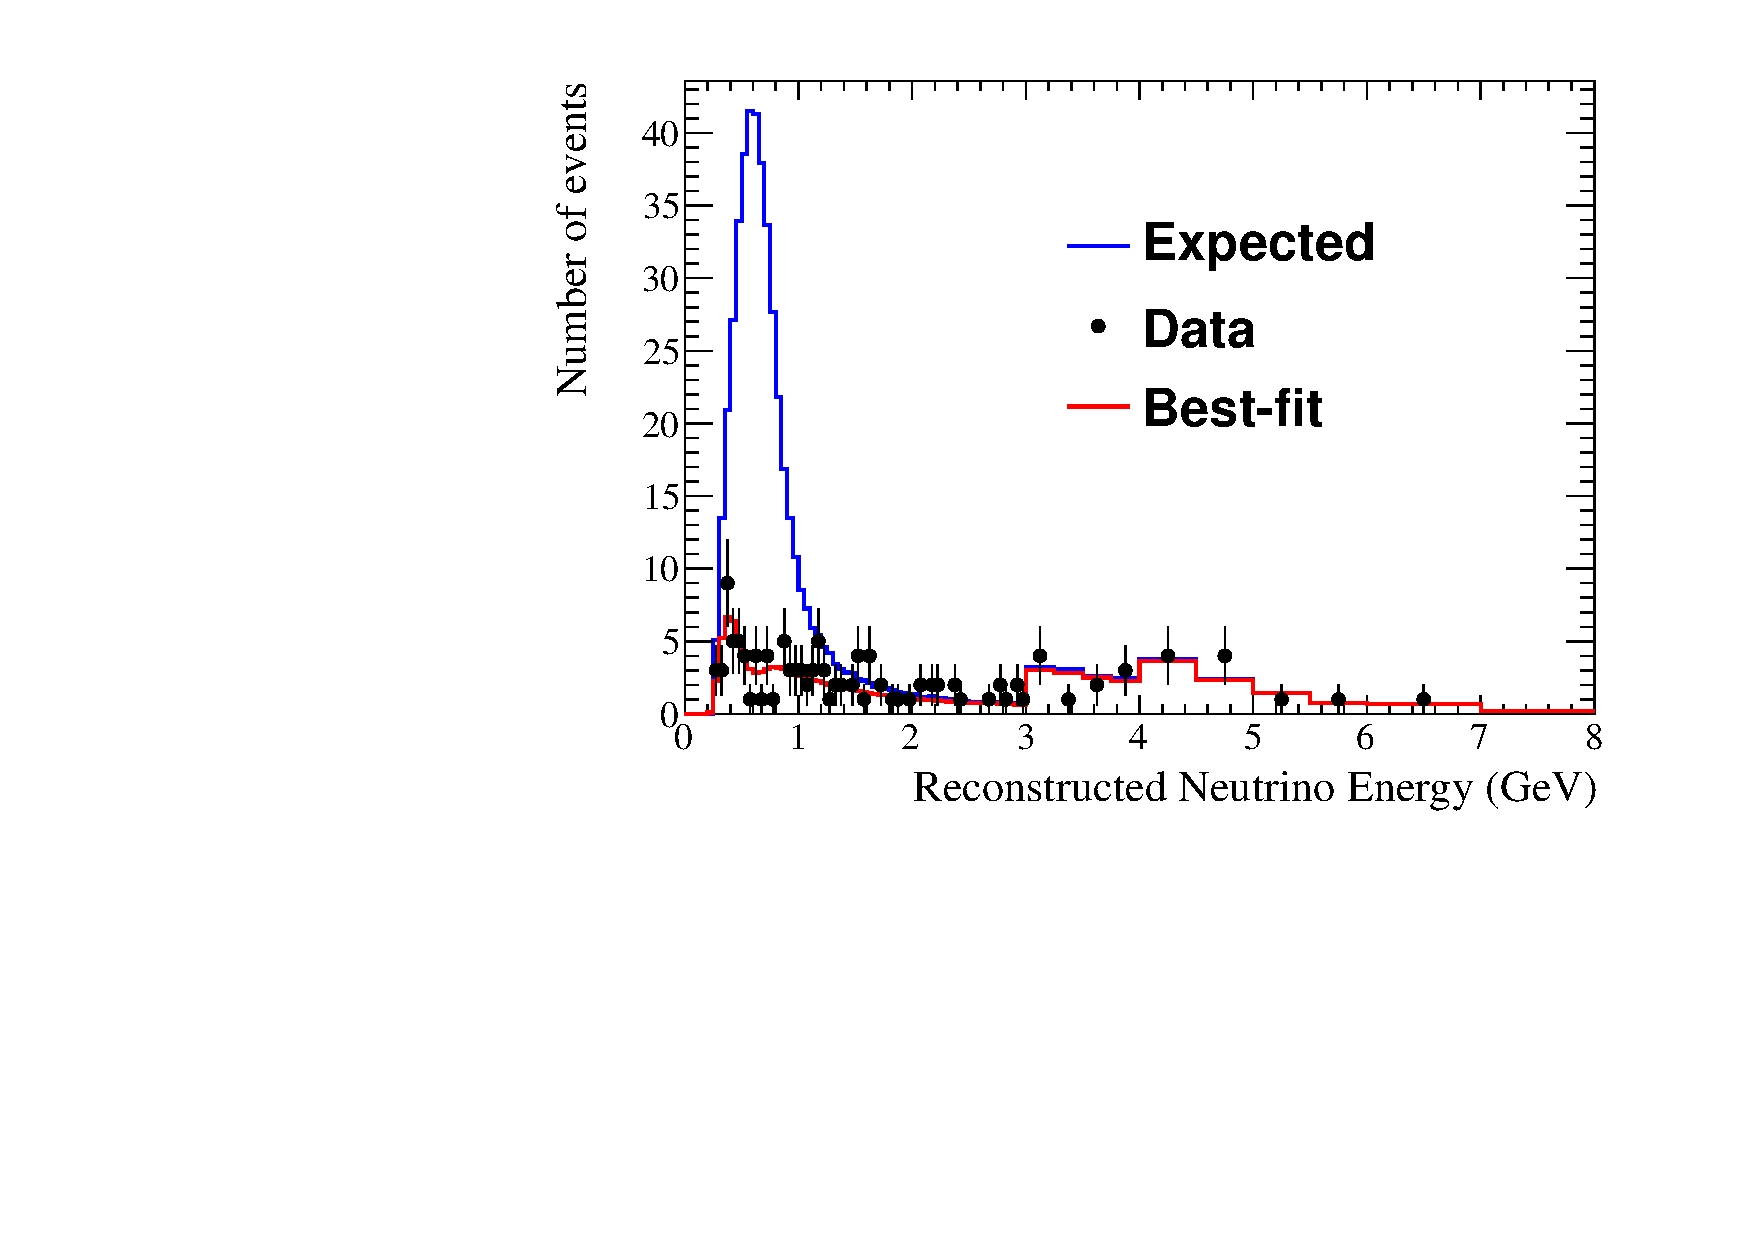
\includegraphics[width=0.9\textwidth]{joint_plots/data/Run17b/bestfit_sinsqth23VsdcpVsMH_1Rmu_Run17.pdf}
\caption{Muon-like, neutrino mode}
\end{subfigure}
\begin{subfigure}[b]{0.49\textwidth}
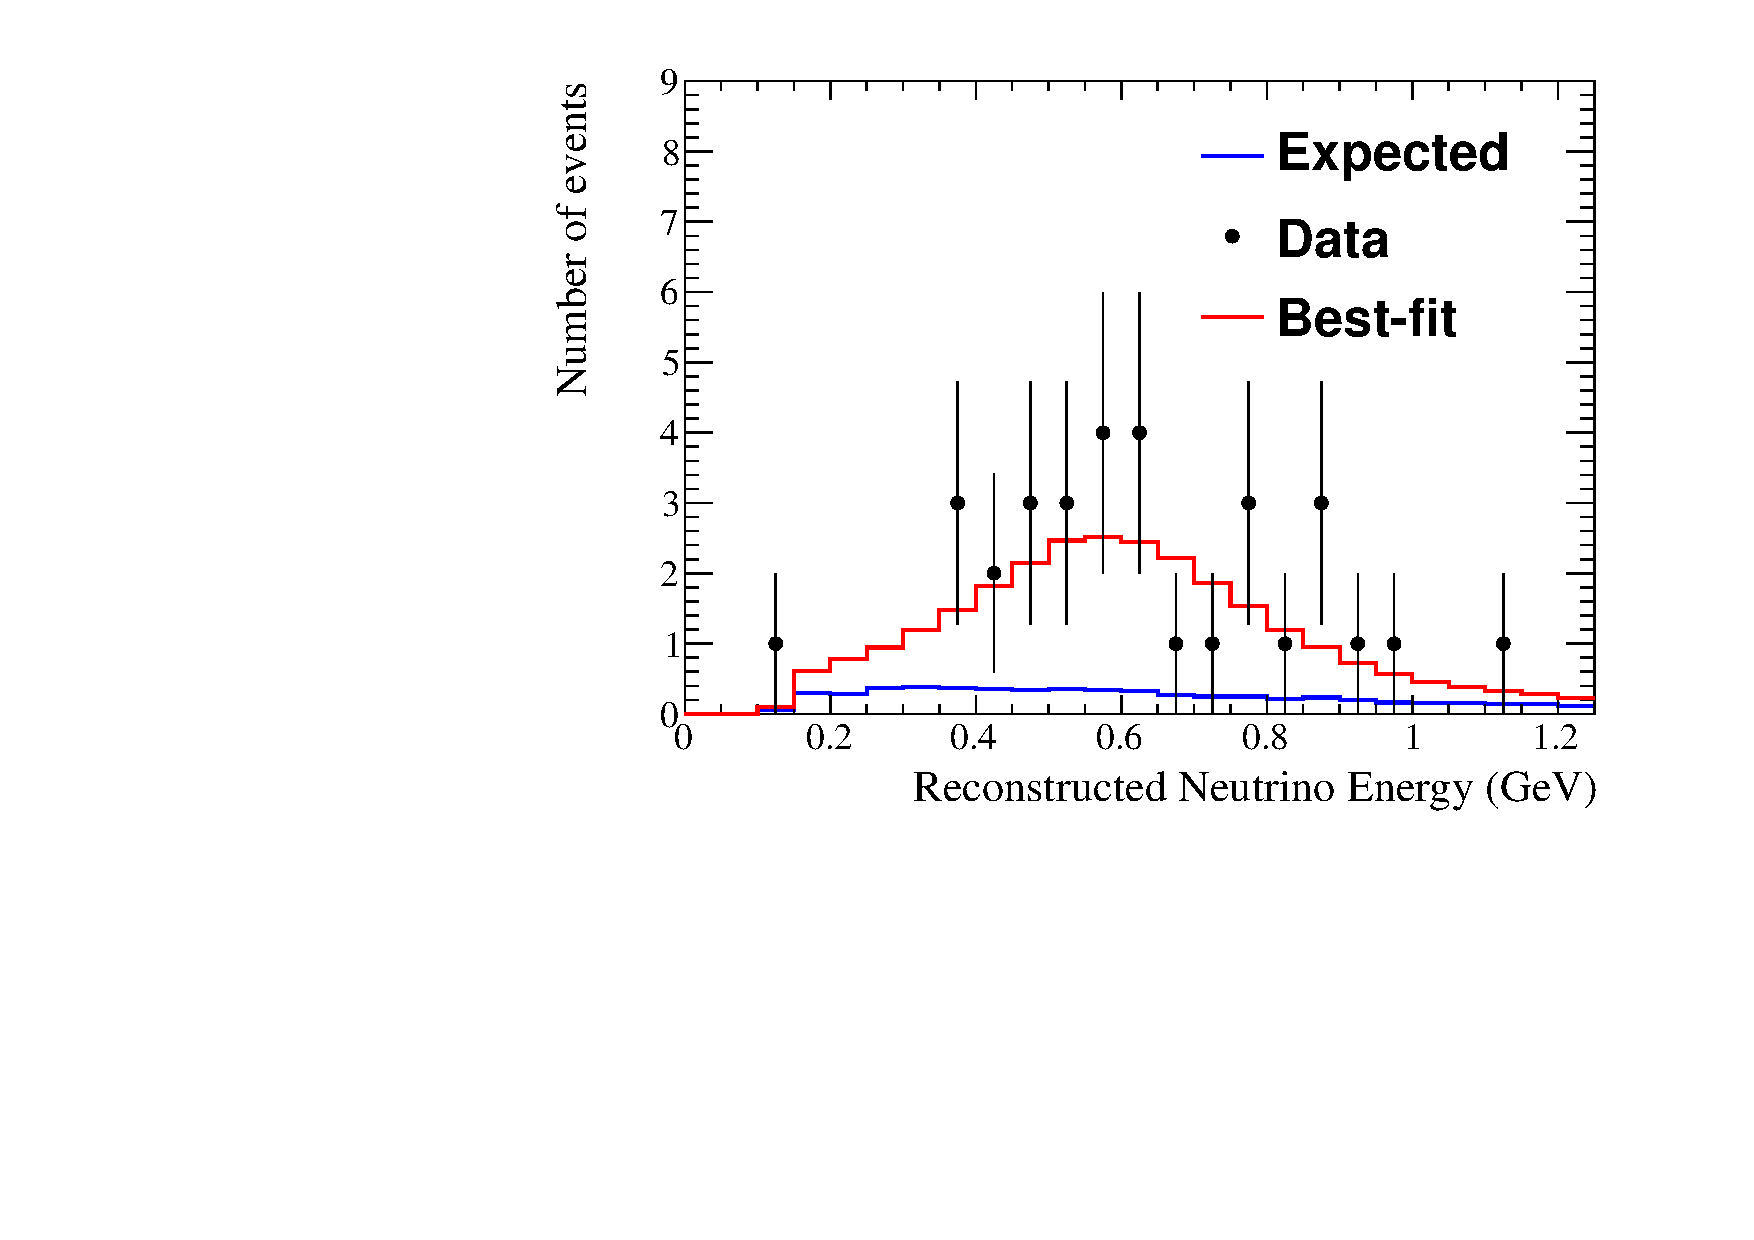
\includegraphics[width=0.9\textwidth]{joint_plots/data/Run17b/bestfit_sinsqth23VsdcpVsMH_1Re_Run17.pdf}
\caption{Electron-like, neutrino mode}
\end{subfigure}
\begin{subfigure}[b]{0.49\textwidth}
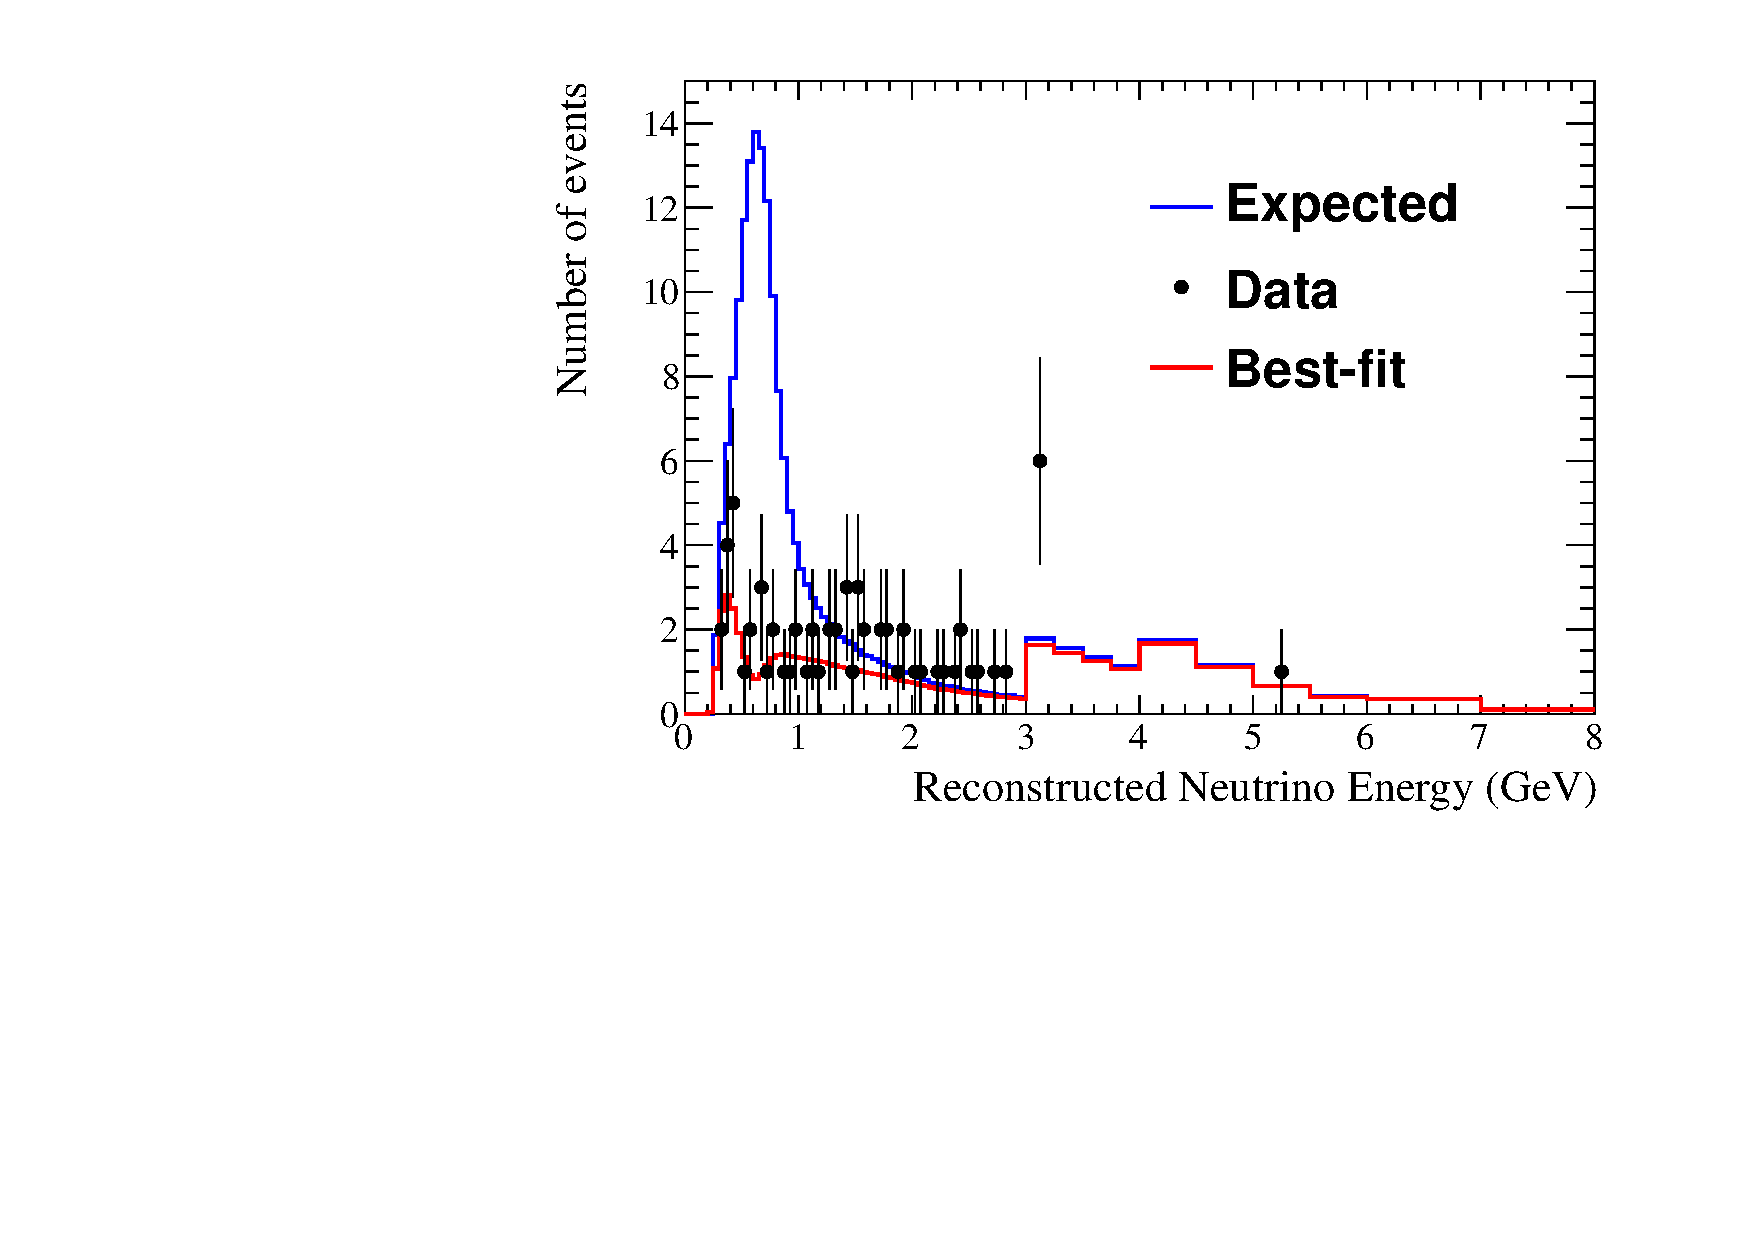
\includegraphics[width=0.9\textwidth]{joint_plots/data/Run17b/bestfit_sinsqth23VsdcpVsMH_RHC1Rmu_Run17.pdf}
\caption{Muon-like, antineutrino mode}
\end{subfigure}
\begin{subfigure}[b]{0.49\textwidth}
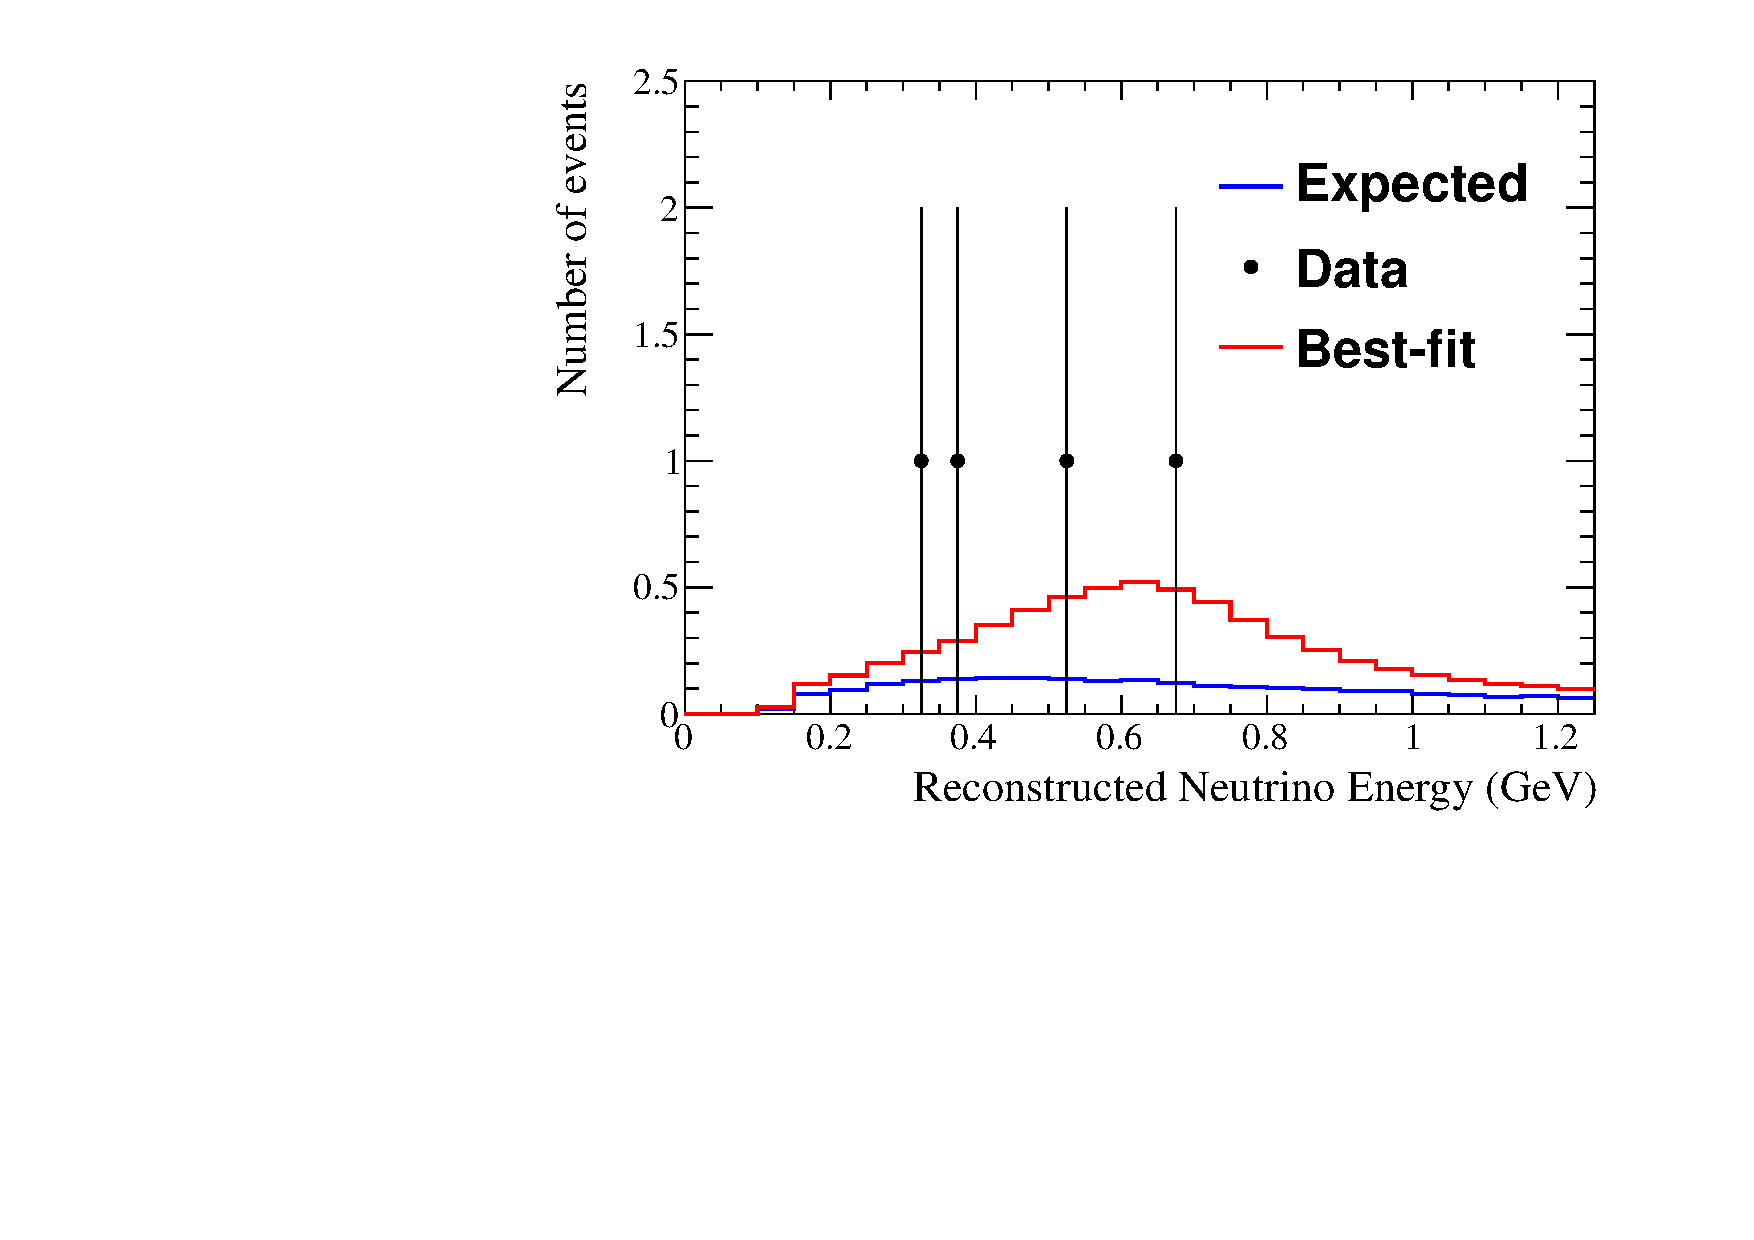
\includegraphics[width=0.9\textwidth]{joint_plots/data/Run17b/bestfit_sinsqth23VsdcpVsMH_RHC1Re_Run17.pdf}
%
\includegraphics[width=0.9\textwidth]{./images/missing_plot-eps-converted-to.pdf}
\caption{Electron-like, antineutrino mode}
\end{subfigure}
\caption {
The best-fit spectra as a function of the neutrino reconstructed energy
are shown for each selected sample
of the Run 1-7b data set.
They correspond to the fit of 
$\sin^2 \theta_{23}$, $\delta_{CP}$ and mass hierarchy 
with reactor constraint
where all the nuisance parameters are marginalised. 
The method described in \cref{eq:bestfit_spectrum_marg} is used.
The best-fit distributions are compared with the 
predicted unoscillated spectrum (all the oscillation parameters are set to 0),
generated with the systematic parameters measured with the ND280 data 
shown in \cref{tab:banff_uncertainties_flux_fhc},
~\ref{tab:banff_uncertainties_flux_rhc},
~\ref{tab:banff_uncertainties_xsec}
and
the nominal Super-K systematic parameters shown in \cref{tab:banff_uncertainties_skdetfsi}.
}
\label{fig:joint_spectra_bf_run17b}
\end{figure*}







% Goodness of fit

A goodness of fit test is performed by comparing data with the best fit spectra shown in \cref{fig:joint_spectra_bf_run17b}.
The same method used for the Run 1-6 data set, shown in \cref{sec:chisq_1d}, is used.
The goodness of fit test has been performed using the same binning as for Run 1-6,
i.e. 5 reconstructed neutrino energy bins (0-0.4, 0.4-0.7, 0.7-1.0, 1.0-2.0 and 2.0-30.0 GeV)
for neutrino mode $\mu$-like and 1 bin for all the other Super-K samples, 
as well as using 5 bins with the same binning as above for both the $\mu$-like samples,
since the antineutrino mode $\mu$-like sample has double of the statistic with Run 1-7b.
At least 6 events are present in each bin.

The $\chi^2$ and resulting p-value for each spectrum is shown in \cref{tab:goodness_of_fit_run17b}. 
We see for all the spectra, the data and best fit spectra are very compatible.

\begin{table}[htb]
\centering
\begin{tabular}{| c | c | c | c |}
\hline
\multicolumn{3}{| c |}{1 bin antineutrino mode $\mu$-like sample}  \\
\hline
Mass Hierarchy d.o.f. 			& $\chi^2$ / ndf        		& p-value \\ \hline
fixed					 		& 3.26785 / 6                  	& 0.77	\\ \hline
free					 		& 3.26785 / 5                 	& 0.66	\\ \hline
\hline
\multicolumn{3}{| c |}{5 bins antineutrino mode $\mu$-like sample}  \\
\hline
Mass Hierarchy d.o.f. 			& $\chi^2$ / ndf        		& p-value \\ \hline
fixed					 		& 4.68245 / 10                  	& 0.91	\\ \hline
free					 		& 4.68245 / 9                 	& 0.86	\\ \hline
\end{tabular}
\caption{
Goodness of fit for the Run 1-7b fit of $\sin^2 \theta_{23}$, $\delta_{CP}$ and mass hierarchy 
where all the other parameters are marginalised. 
Since the mass hierarchy is a discrete parameter, the goodness of the fit test 
is performed assuming the mass hierarchy both as a free parameter and as a fixed parameter.
$ndf = 5$ if the mass hierarchy is assumed to behave as 1 degree of freedom.
The test is performed with both 1 and 5 reconstructed neutrino energy bins for 
antineutrino mode $\mu$-like sample.
}
\label{tab:goodness_of_fit_run17b}
\end{table}



%--------------------------------------------------------------------------------------
%
% Feldman-Cousins deltaCP Vs mh
%
%--------------------------------------------------------------------------------------

\subsection {Feldman-Cousins and significance for the simultaneous fit of $\delta_{CP}$ and mass hierarchy for Run 1-7b}
\label{sec:fc_significance_run17b}


In \cref{fig:joint_dcp_fc_run17b} the confidence intervals obtained with the ``Feldman-Cousins" method
are shown for $\delta_{CP}$ and mass hierarchy with reactor constraint for the Run 1-7b data set.
The critical values at both 90\% and $2\sigma$ CL are computed
for both the mass hierarchies and the following true values of $\delta_{CP}$: 
$-\pi$, -2.356, $-\pi/2$, -0.785, 0, +0.785, $+\pi/2$, -2.356, $+\pi$. 
The procedure described in \cref{sec:cl} is used.
The $\pm 1 \sigma$ error on the critical values are shown as well.
The same procedure used for the Run 1-6 data fit, shown in \cref{sec:fc_significance}, is used.
Inverted hierarchy is almost excluded at 90\% CL except for a small interval around $\delta_{CP} = -\pi / 2$.
$\delta_{CP} = 0$ is still disfavored with respect to $\delta_{CP} = \pi$, which, however, is excluded at 90\% CL. 
We can say that CP conservation assuming the PMNS framework is excluded at 90\% CL. 

\begin{figure*}[htb]
\center
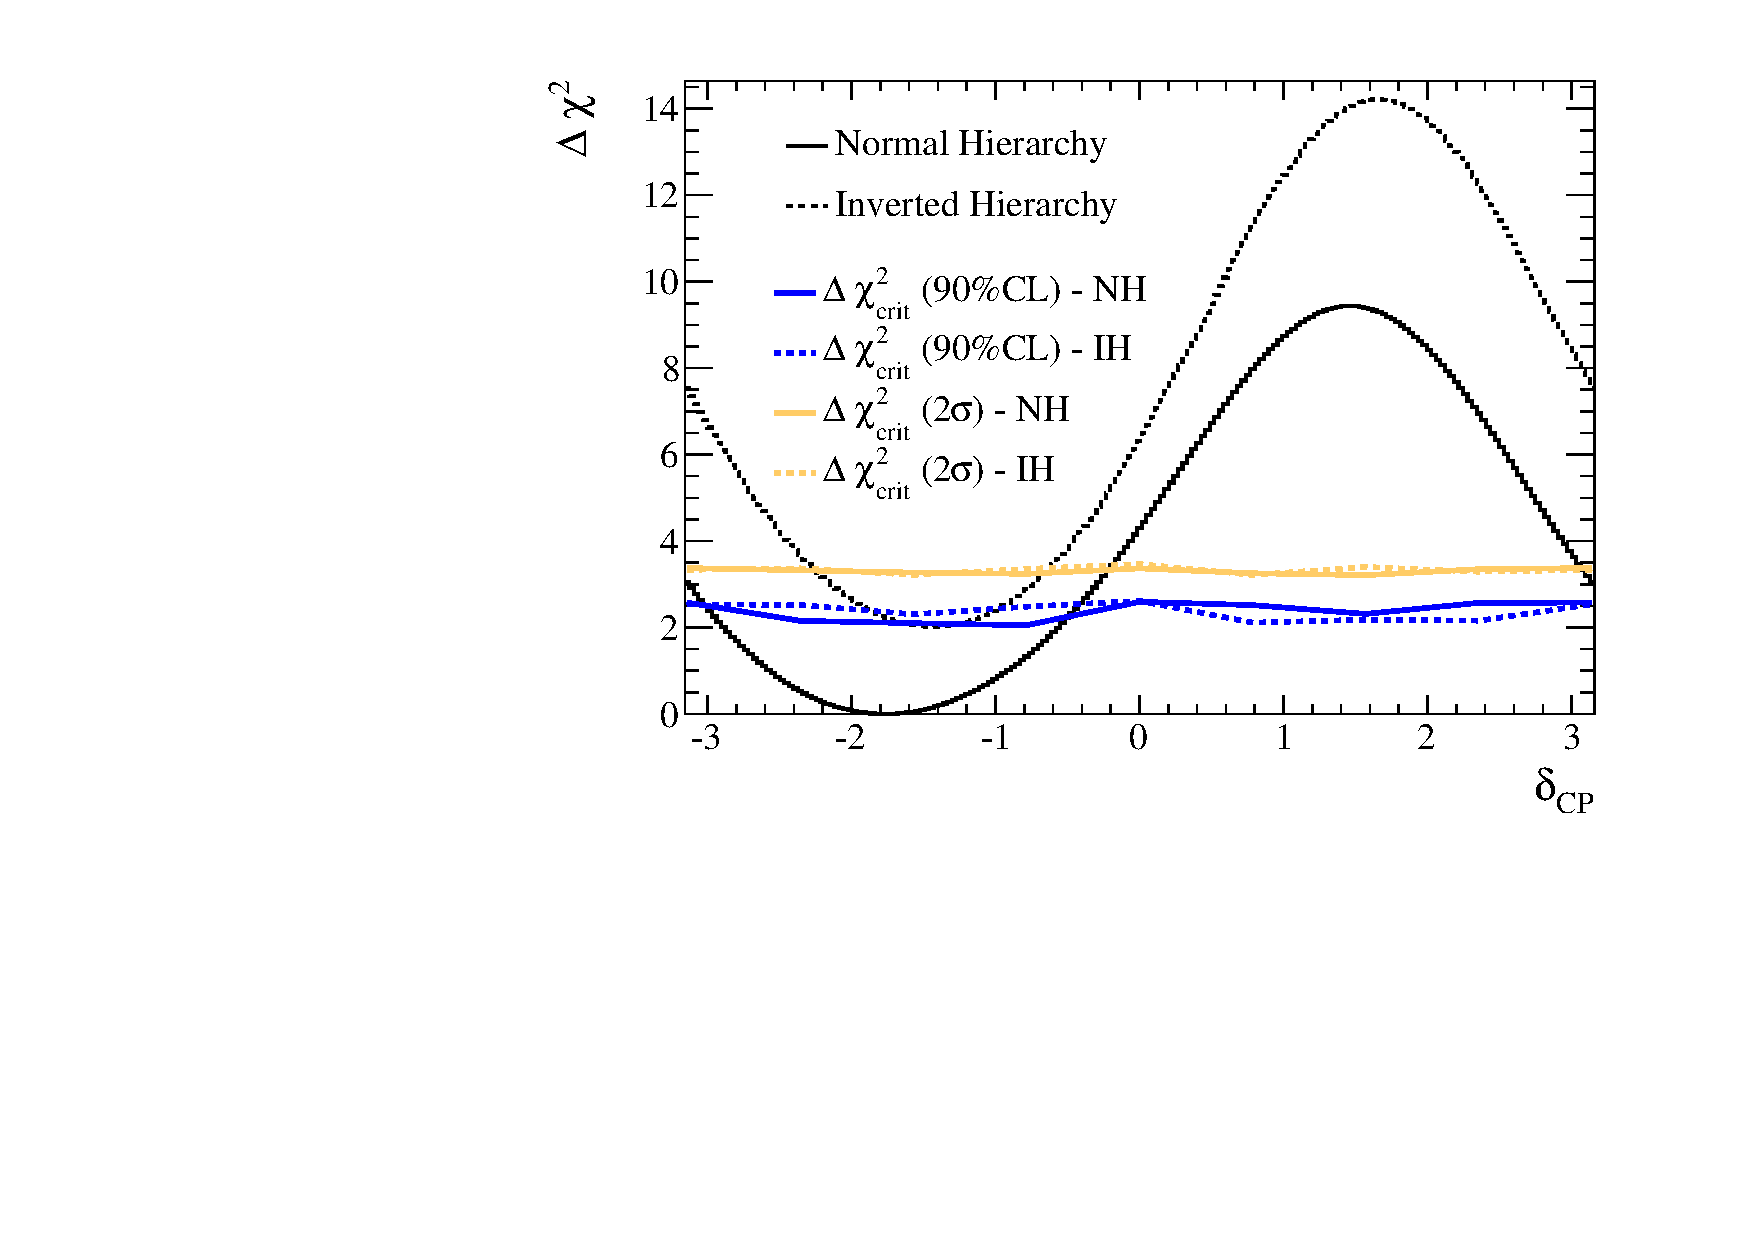
\includegraphics[width=0.49\textwidth]{joint_plots/coverage_fc/fc_run17b/dcp_mh_react_run17.pdf} 
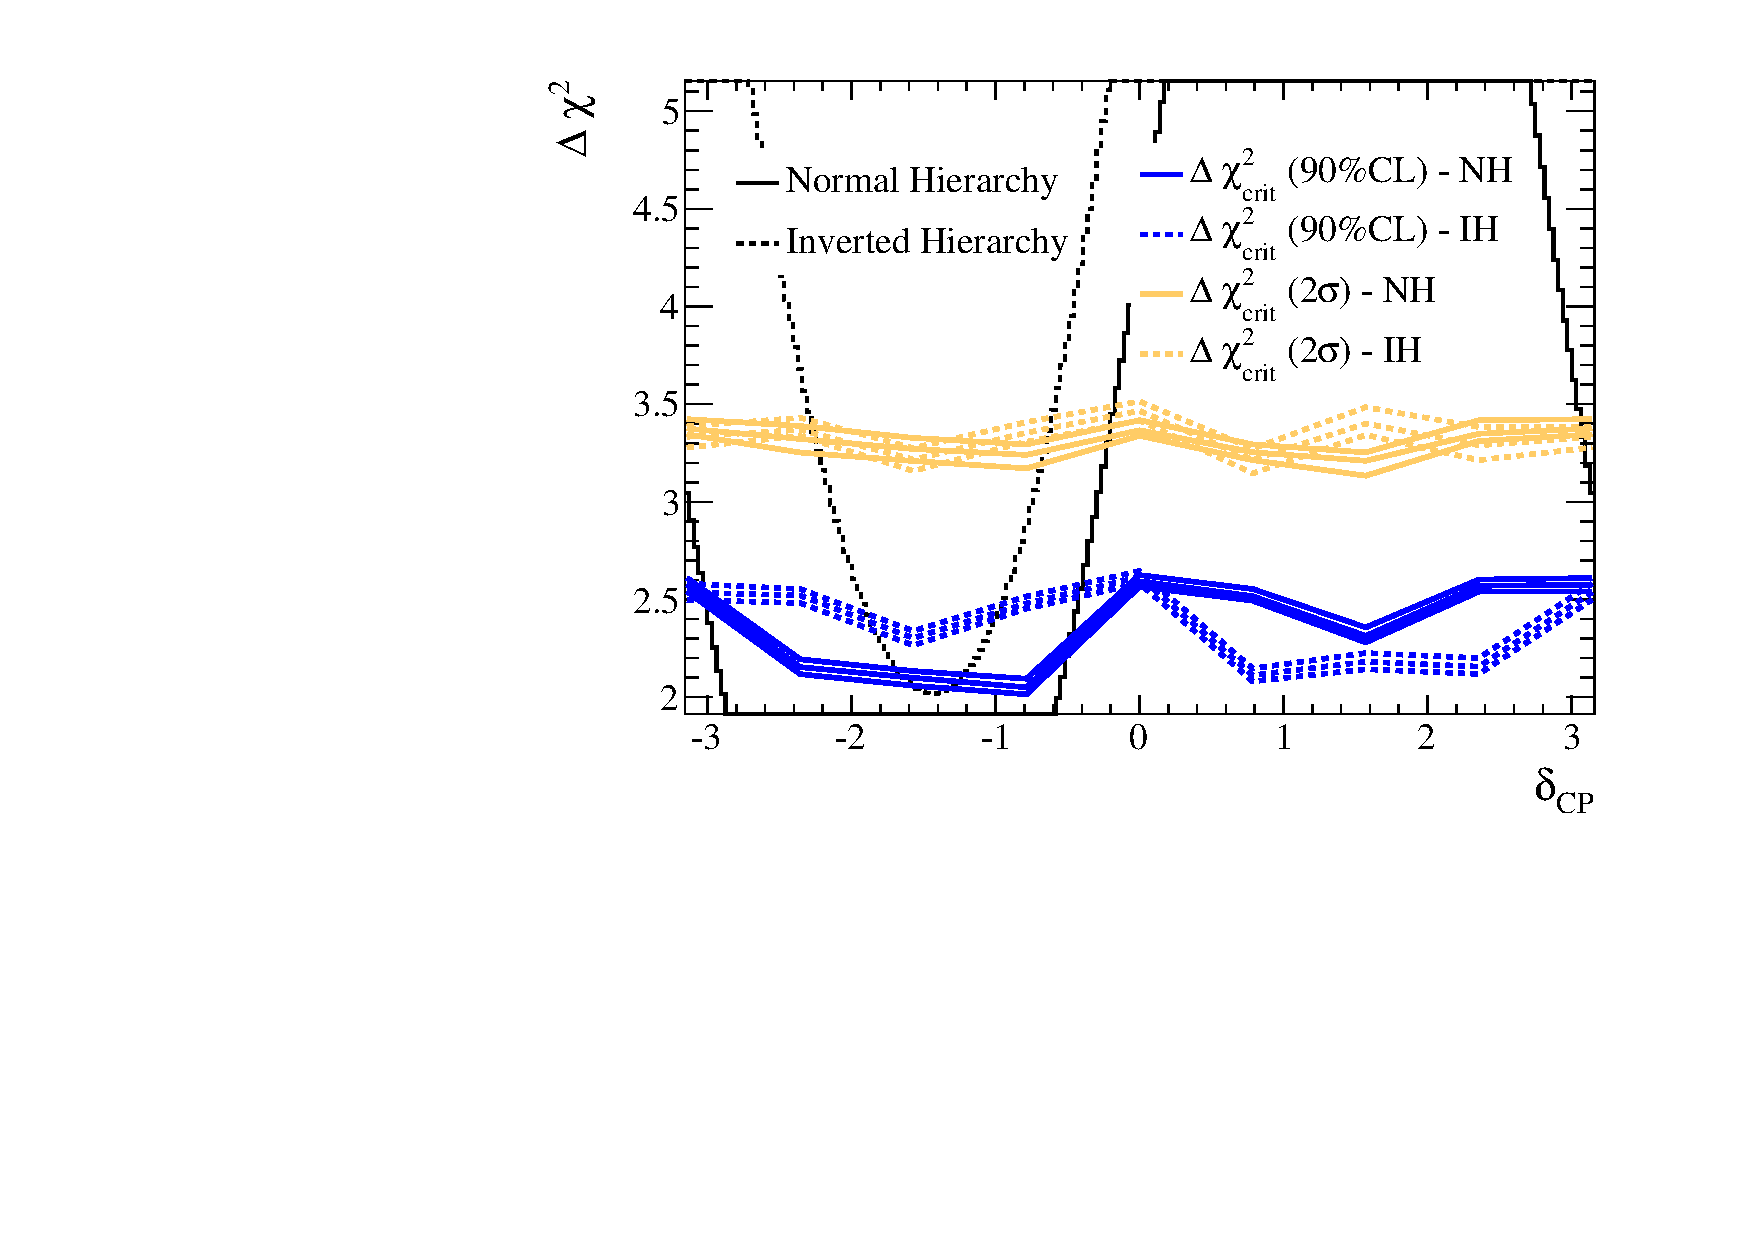
\includegraphics[width=0.49\textwidth]{joint_plots/coverage_fc/fc_run17b/dcp_mh_react_run17_zoom.pdf} 
\caption{
Measured $\Delta \chi^2$ distributions with the full Run 1-7b data set.
Both normal (black solid line) and inverted (black dashed line) hierarchies are shown. 
The ``Feldman-Cousins" method is used to set the $\Delta \chi^2$ critical values in order to provide 
confidence intervals with the proper coverage.
The ranges of $\delta_{CP}$ which correspond to $\Delta \chi^2$ values larger than the critical 
values (blue for 90\% CL and orange for $2\sigma$ CL) are excluded at a certain confidence level.
Both normal and inverted hierarchy $\Delta \chi^2$ distributions are shifted with respect to the same global minimum. 
All the oscillation parameters which are not parameters of interest
are marginalised using the prior distributions shown in \cref{tab:marg_binnning}.
The $\pm1 \sigma$ error on the critical values is shown as well, where specified, 
and is represented by the lowest and highest set of critical values, with the same color of the central ones.
On the right plot a zoom on the critical values is shown.
}
\label{fig:joint_dcp_fc_run17b}
\end{figure*}

























%--------------------------------------------------------------------------------------
%
% Contours
%
%--------------------------------------------------------------------------------------

\subsection {2-dimensional confidence intervals}
\label{sec:results_2d_contours_run17b}

The same 2-dimensional confidence intervals as in \cref{sec:results_2d_contours} are produced.
In \cref{fig:joint_sensi_t2krun14bf_2d_run17b} the corresponding 2-dimensional contours produced
with the Run 1-7b data set are shown drawing the normal and inverted hierarchy contours independently,
i.e. each contour is produced with respect to the global minimum under that hierarchy hypothesis.
%In \cref{fig:joint_sensi_t2krun14bf_2d_glob} both normal and inverted hierarchy contours
%are produced with respect to the same global minimum, i.e. the normal hierarchy hypothesis.
%As already explained in \cref{sec:cl_mh}, ``global" and ``independent" contours correspond
%respectively to the least and most conservative approach.

As in 1-dimensional analysis results
in \cref{fig:joint_data_fit_1d_run17b}, the reactor measurements are 
in agreement with the T2K data at $1\sigma$ level if $\delta_{CP} \sim - \frac{\pi}{2}$. 
Compared to \cref{fig:joint_sensi_t2krun14bf_2d}, both the normal and inverted 
hierarchy contours are closer to the reactor measurement.
Furthermore we can see that the region close $\delta_{CP} = + \pi/2$ is excluded at 90\% CL.

The other contours are similar to the Run 1-6 data set ones.

%As a result, we see that all $\delta_{CP}$ constraints in 
%\cref{fig:ss13_dcp_with_reactor_data_fit},~\ref{fig:dmsq_dcp_with_reactor_data_fit},~\ref{fig:ss23_dcp_with_reactor_data_fit} 
%are tighter for the inverted hierarchy hypothesis than for the normal.
%\cref{fig:dmsq_dcp_with_reactor_data_fit} also shows a slight anti-correlation between $\delta_{CP}$ 
%and $\Delta m^2_{32}$ in the normal hierarchy fit and a correlation in the inverted most likely coming 
%from the fact that $\Delta m^2_{32}$ and $cos(\delta_{CP})$ have similar effects on the shape of the appearance spectra. 
%In \cref{fig:ss23_dcp_with_reactor_data_fit} we see correlation where the constraint on $\delta_{CP}$ is narrower 
%for smaller values of $\sin^2 \theta_{23}$ as they both appear in the appearance term. 
%In \cref{fig:ss23_dmsq_with_reactor_data_fit} we see that $\sin^2 \theta_{23}$ and $\Delta m^2_{32}$ 
%are not very correlated however the inverted hierarchy contour is shifted down in $\Delta m^2_{32}$ 
%with respect to the normal hierarchy contour. 
%This effect is due to the correlation between $\Delta m^2_{32}$ and the mass hierarchy shown in \cref{fig:mass_hierarchy_MC_shift}. 
%Indeed the inverted hierarchy hypothesis produces an event migration toward higher energy 
%which is balanced in the fit by a lower fit value of $\Delta m^2_{13}$ with respect to the normal hierarchy case.

\begin{figure*}[htb]
\center
\begin{subfigure}[b]{0.49\textwidth}
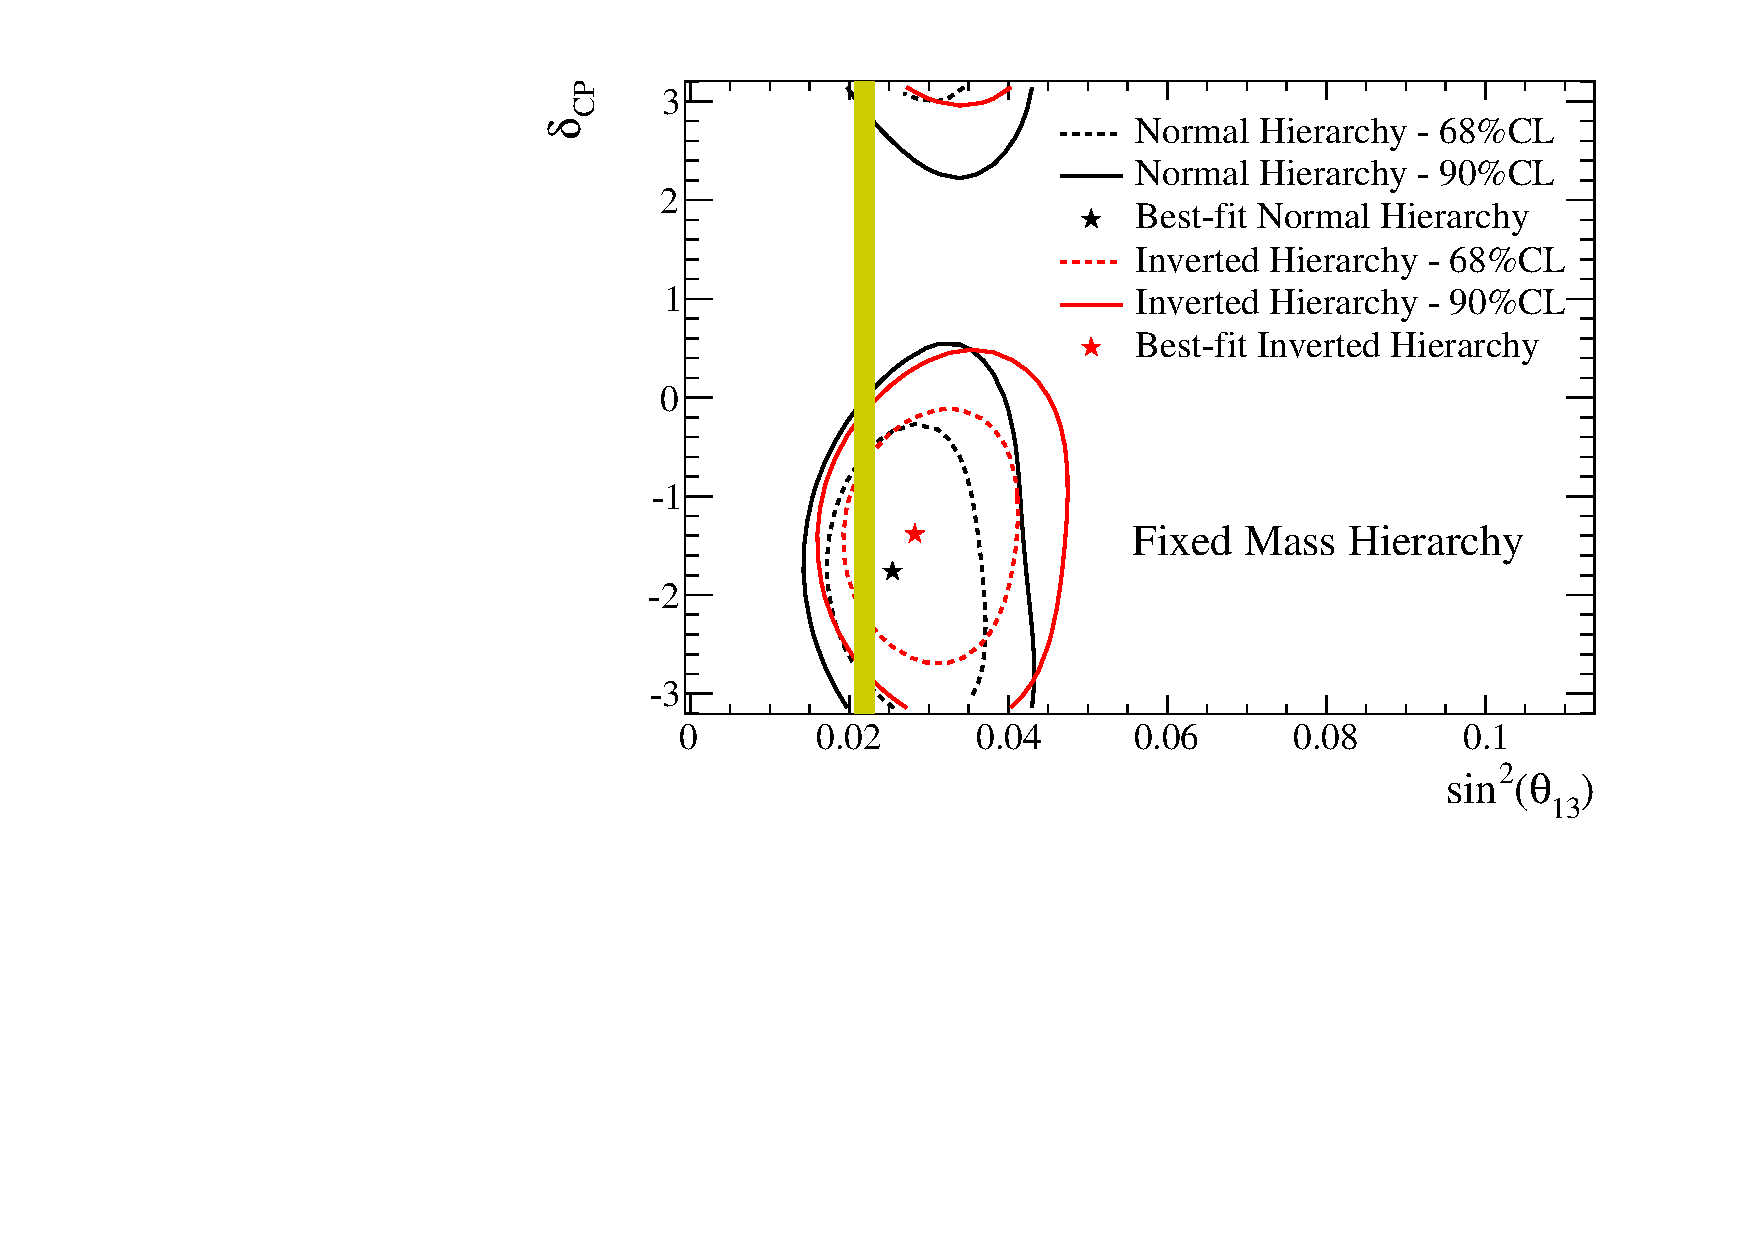
\includegraphics[width=0.9\textwidth]{joint_plots/data_contours/Run17b/sinsqth13Vsdcp_t2konly_run17_constdchisq.pdf}
\caption{$\sin^2 \theta_{13}$ vs $\delta_{CP}$ with T2K data only}
\label{fig:ss13_dcp_t2k_only_data_fit_run17b}
\end{subfigure}
\begin{subfigure}[b]{0.49\textwidth}
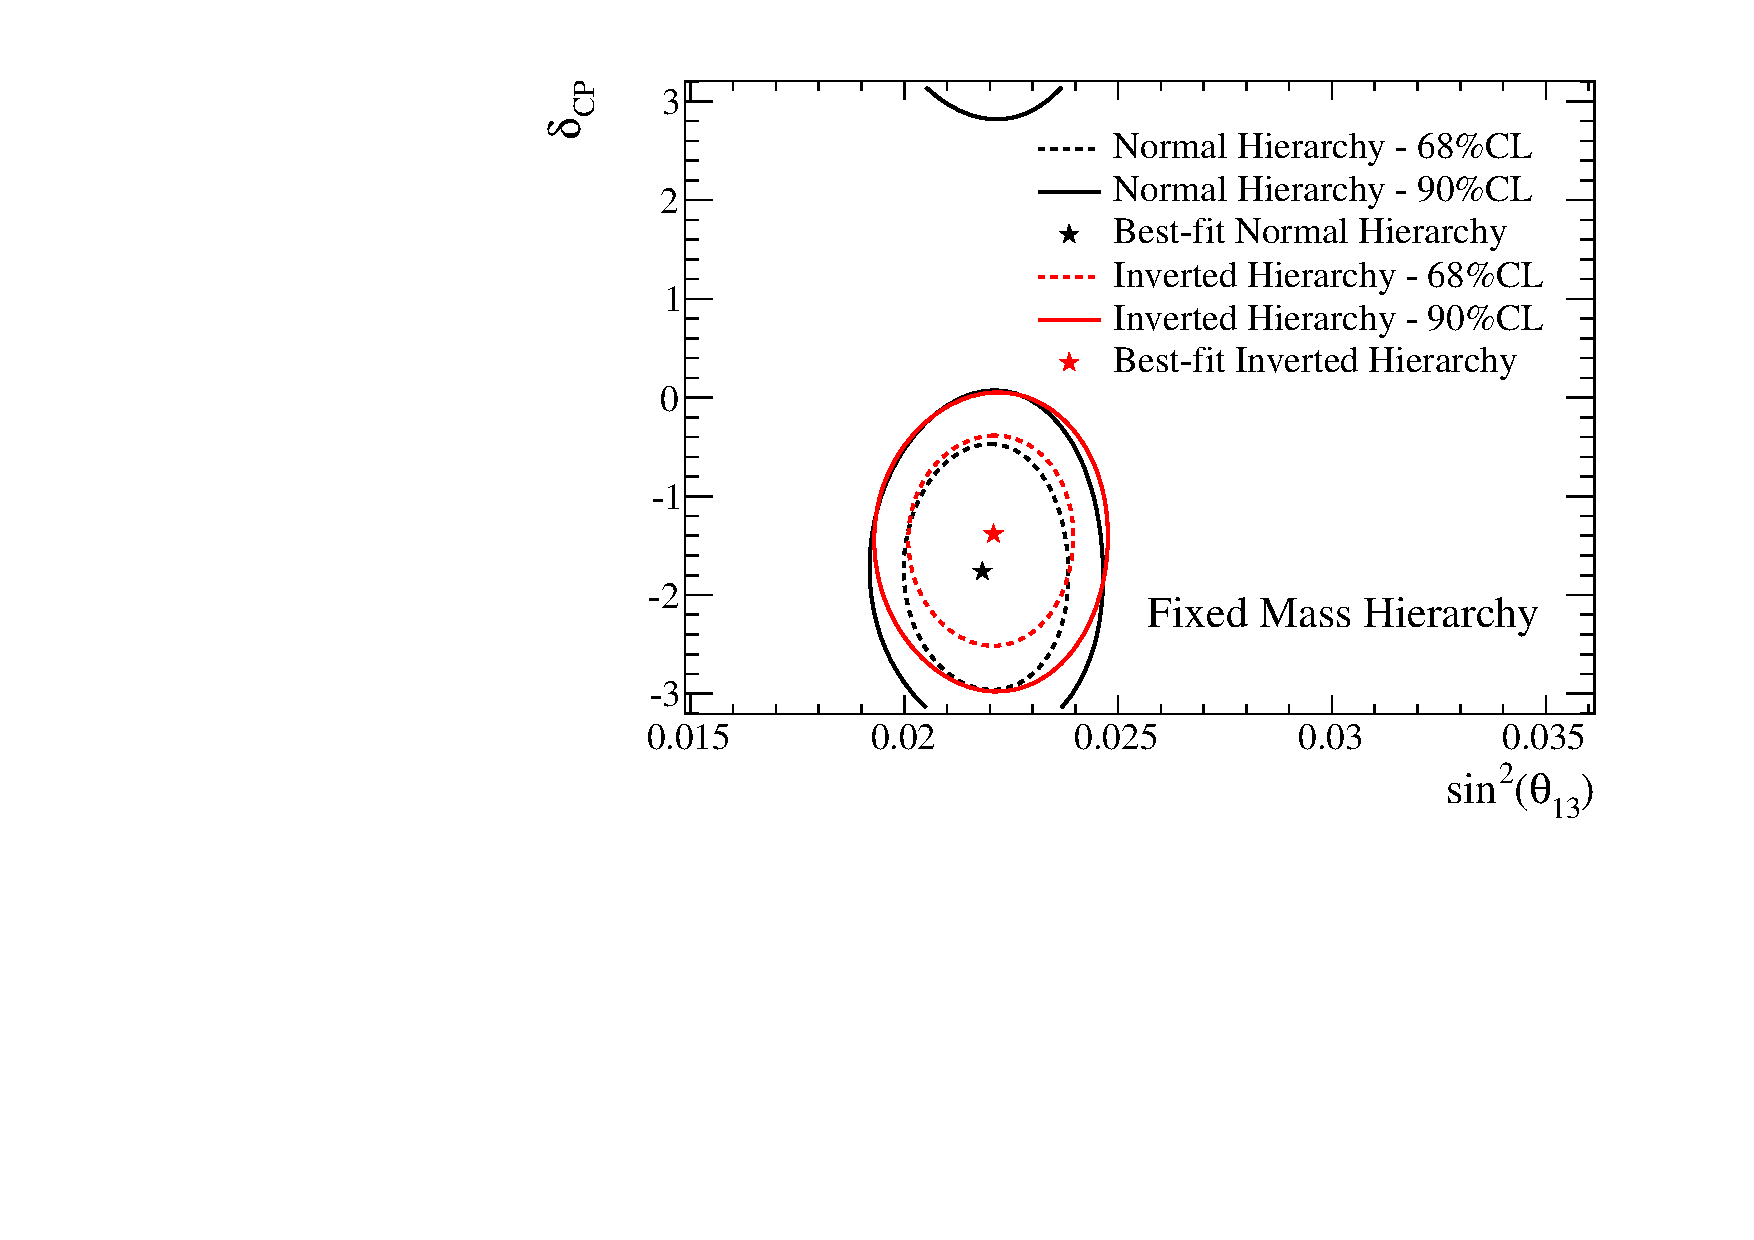
\includegraphics[width=0.9\textwidth]{joint_plots/data_contours/Run17b/sinsqth13Vsdcp_react_run17_constdchisq.pdf}
\caption{$\sin^2 \theta_{13}$ vs $\delta_{CP}$ with reactor constraint}
\label{fig:ss13_dcp_with_reactor_data_fit_run17b}
\end{subfigure}
\begin{subfigure}[b]{0.49\textwidth}
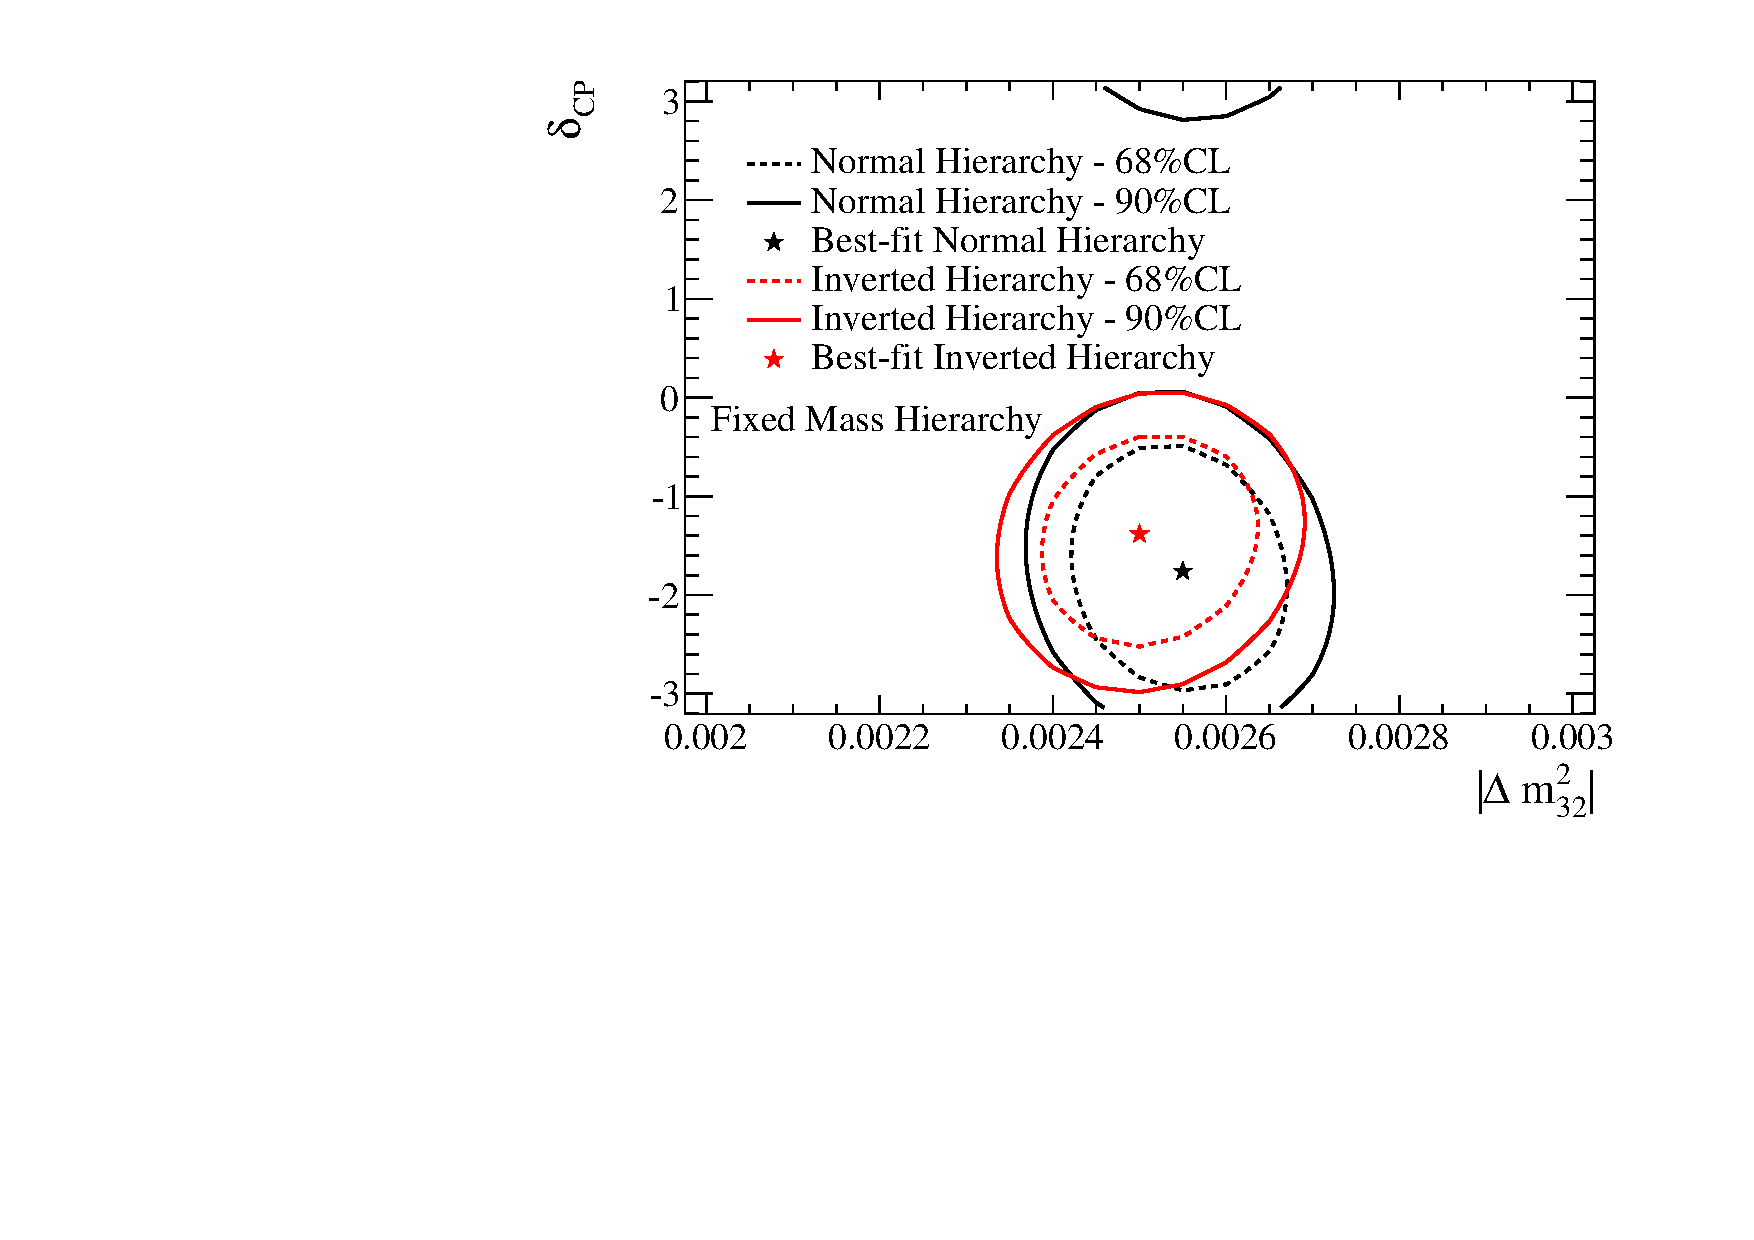
\includegraphics[width=0.9\textwidth]{joint_plots/data_contours/Run17b/dmsqVsdcp_react_run17_constdchisq.pdf}
\caption{$\Delta m^2_{32}$ ($\Delta m^2_{13}$) vs $\delta_{CP}$ with reactor constraint}
\label{fig:dmsq_dcp_with_reactor_data_fit_run17b}
\end{subfigure}
\begin{subfigure}[b]{0.49\textwidth}
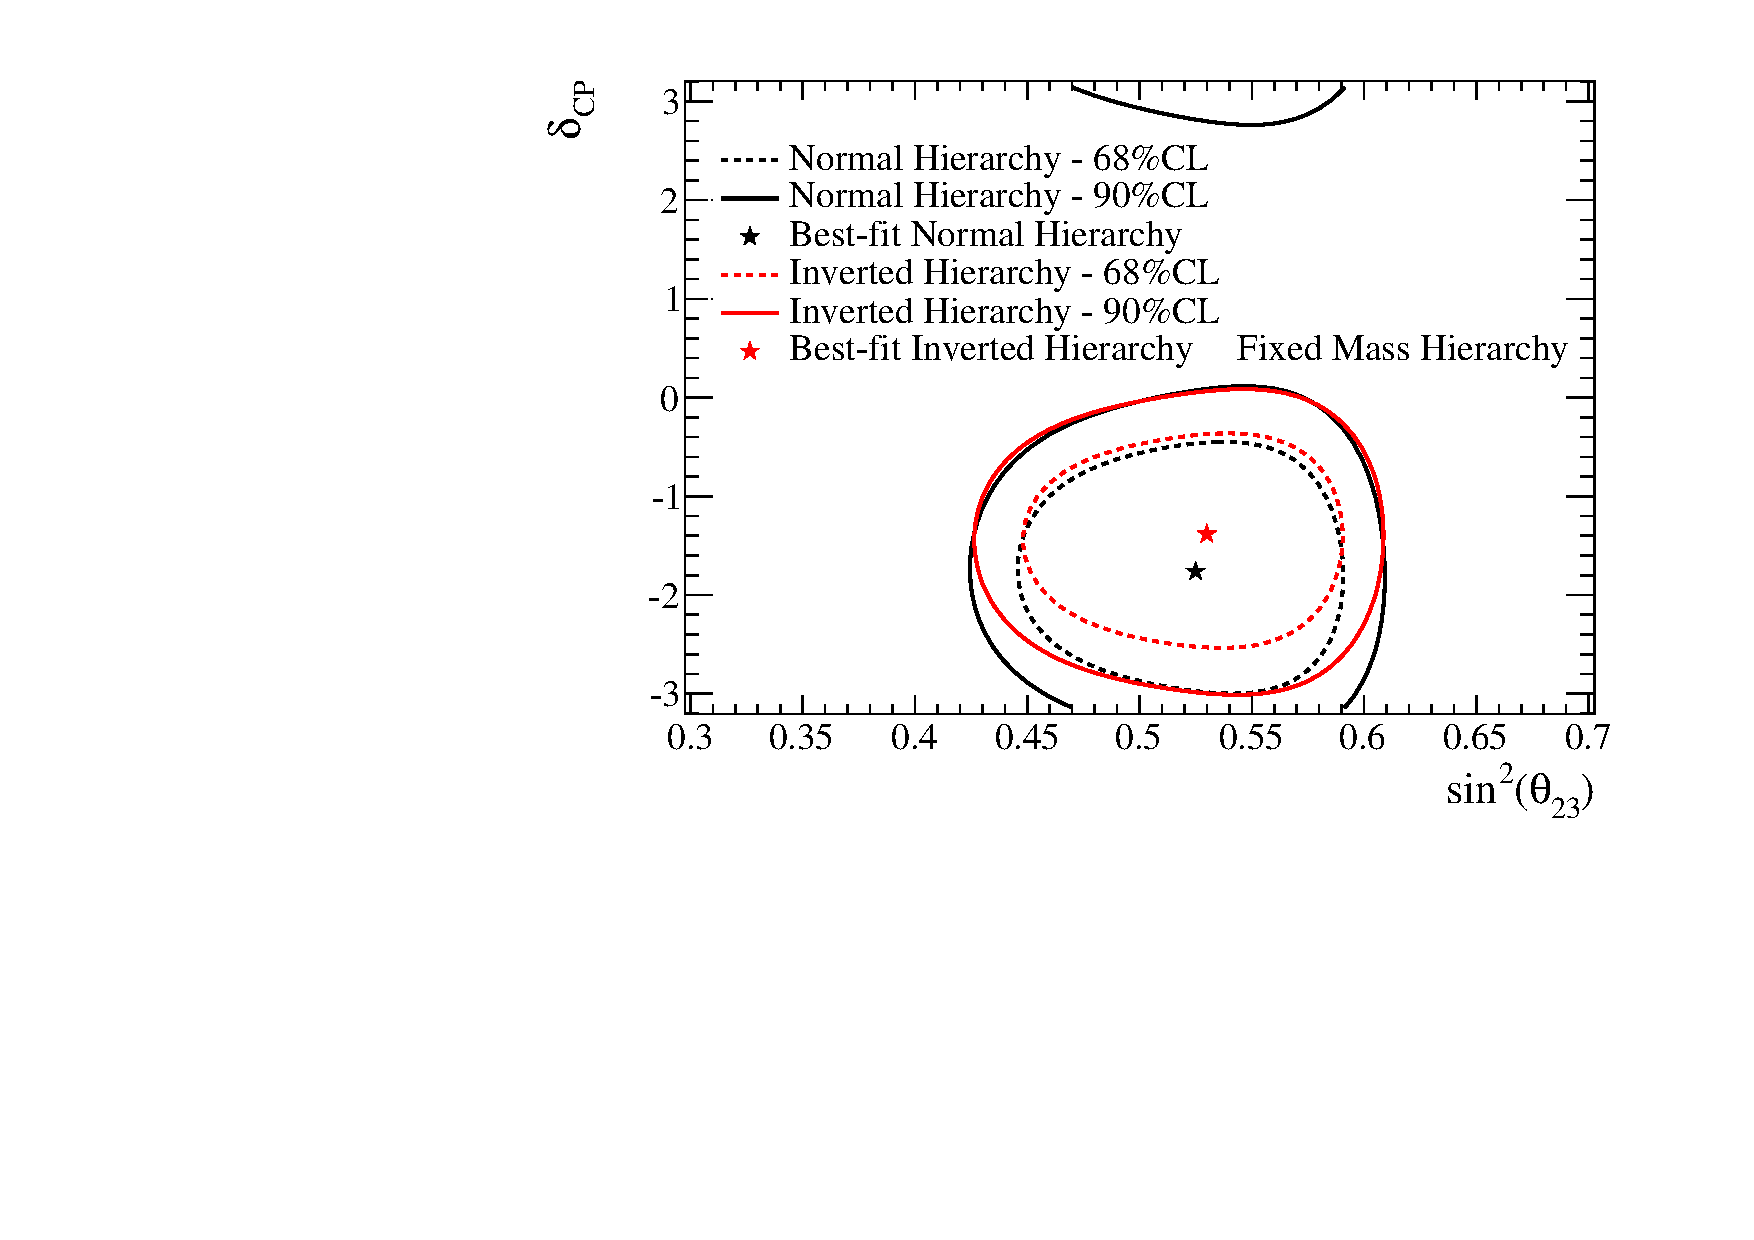
\includegraphics[width=0.9\textwidth]{joint_plots/data_contours/Run17b/sinsqth23Vsdcp_react_run17_constdchisq.pdf}
\caption{$\sin^2 \theta_{23}$ vs $\delta_{CP}$ with reactor constraint}
\label{fig:ss23_dcp_with_reactor_data_fit_run17b}
\end{subfigure}
\begin{subfigure}[b]{0.49\textwidth}
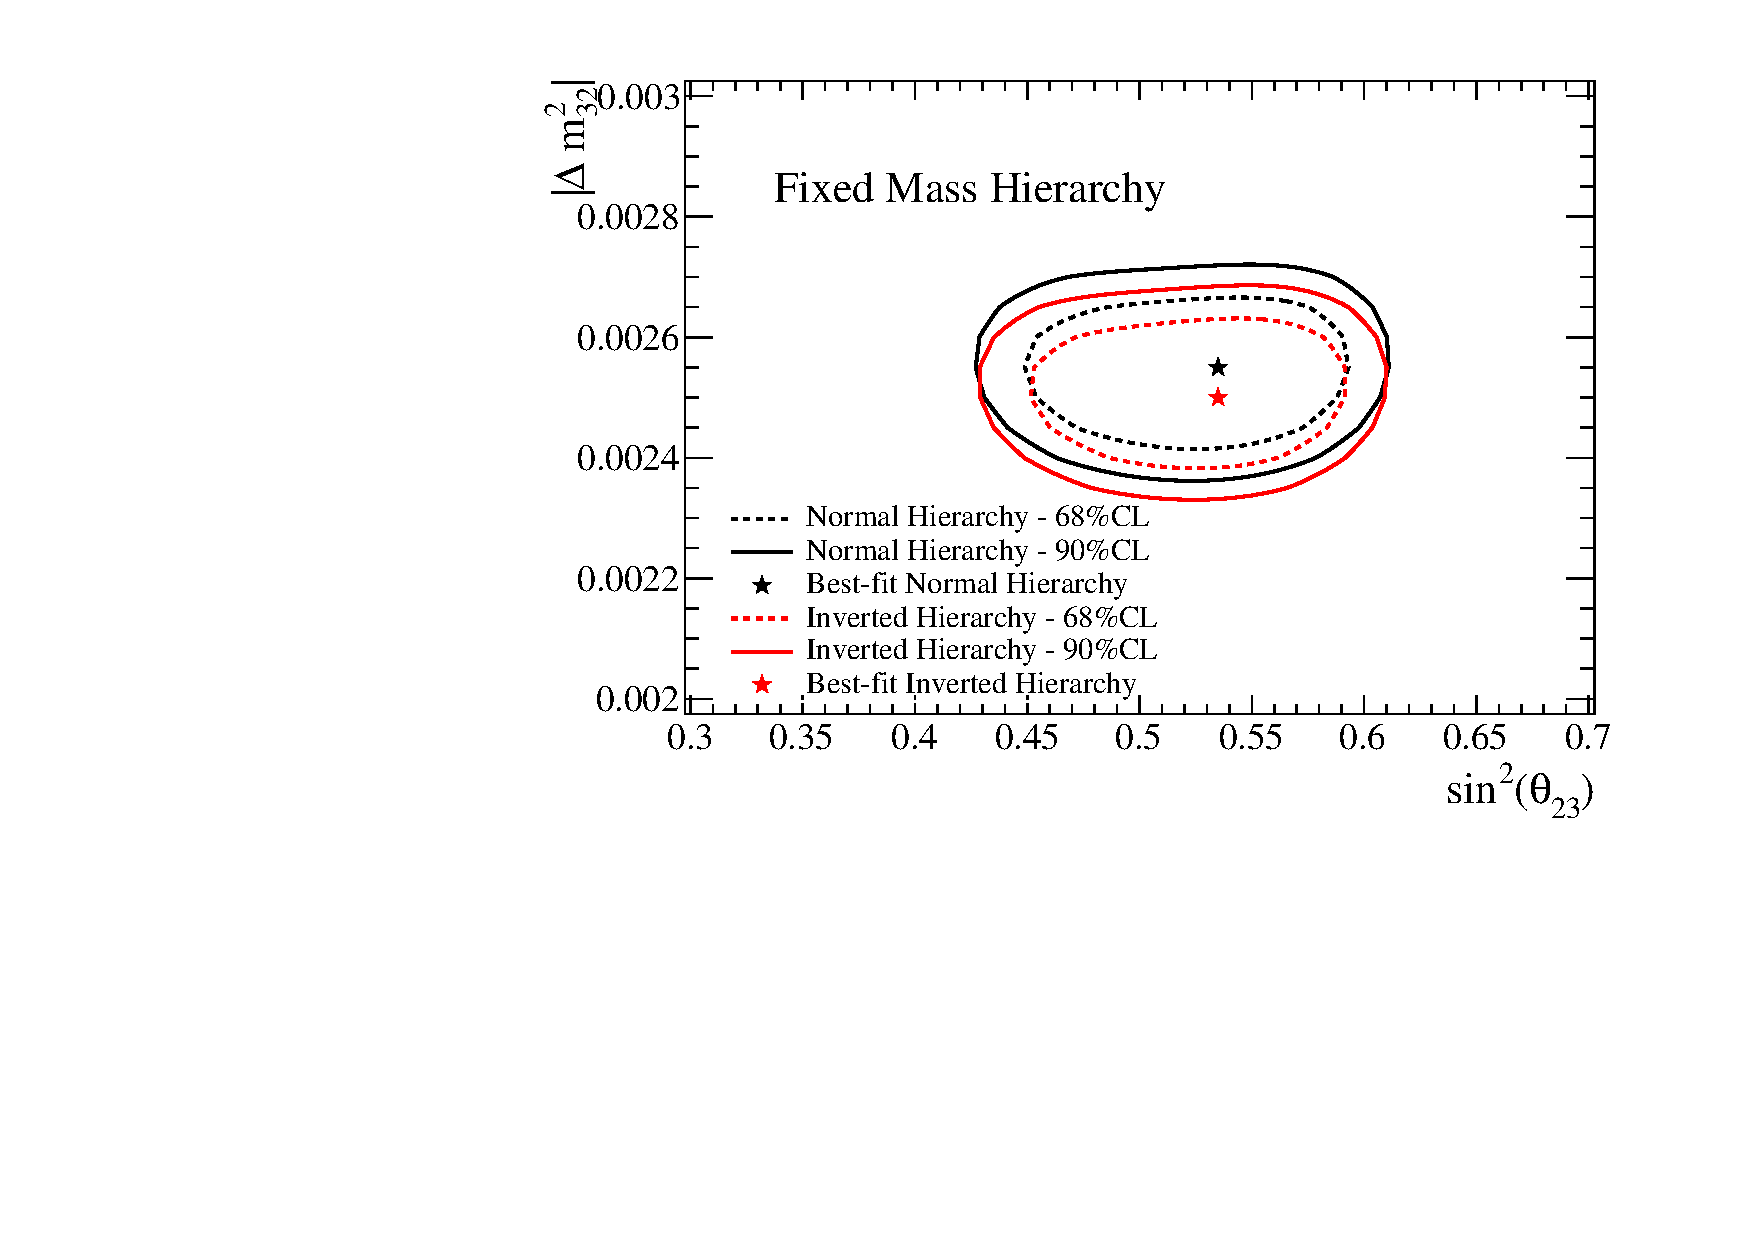
\includegraphics[width=0.9\textwidth]{joint_plots/data_contours/Run17b/sinsqth23Vsdmsq_react_run17_constdchisq.pdf}
\caption{$\sin^2 \theta_{23}$ vs $\Delta m^2_{32}$ ($\Delta m^2_{13}$)
with reactor constraint}
\label{fig:ss23_dmsq_with_reactor_data_fit_run17b}
\end{subfigure}
\caption{
%{\large{MEASURED 2D CONTOURS}}
Measured confidence intervals with the full Run 1-7b data set.
Both normal (black) and inverted (red) hierarchies are shown. 
Both 68\% (dashed line) and 90\% CL (solid line) are shown.
Confidence intervals are produced using the \emph{constant} $\Delta \chi^2$ method. % (see \cref{app:method_cl}).
Contours for normal (black) and inverted (red) hierarchy are computed independently.
All the oscillation parameters which are not parameters of interest
are marginalised using the prior distributions shown in \cref{tab:osc_params_joint_priors}.
The measured contour of $\sin^2 \theta_{13}$ vs $\delta_{CP}$ without reactor constraint, in \cref{fig:ss13_dcp_t2k_only_data_fit} is compared with the measurement by reactor experiments, 
$\sin^2 \theta_{13} = 0.0219 \pm 0.0012 $
\cite{pdg_2014},
shown by the yellow bar.
}
\label{fig:joint_sensi_t2krun14bf_2d_run17b}
\end{figure*}



\clearpage






%%...........................................................
%%
%% Comparison of Run 1-7 data with sensitivity
%%
%%...........................................................
%
%\subsection {Comparison of $\delta_{CP}$ vs mass hierarchy Run 1-7 result with sensitivity}
%\label{sec:comparison_data_sensi_dcp_run17}
%
%In order to understand better the output of the Run 1-7 data fit, the result 
%has been compared with the expected sensitivity obtained by performing 10k toy experiments
%for different true values of $\delta_{CP}$ and mass hierarchy.
%
%\subsubsection {$\delta_{CP} = -\pi/2$ - normal hierarchy}
%\label{sec:dcp_mpiover2_nh_run17}
%
%In \cref{fig:brazilian_mpiover2_run17} the Run 1-7 data result for $\delta_{CP}$ vs mass hierarchy 
%is compared to the expected mean $\Delta \chi^2$ ($<\Delta \chi^2>$)
%distribution as well as the $1\sigma$ and $2\sigma$ 
%uncertainties on the $\Delta \chi^2$ distributions
%corresponding to $\delta_{CP}=-\pi/2$ and normal hierarchy.
%
%The sensitivity plot was obtained as following:
%\begin{itemize}
%
%\item 10k toy experiments were performed for $\delta_{CP} = -\pi/2$ and normal hierarchy
%	and the full $\chi^2_{toy}$ was computed as described in \cref{sec:marginalization}.
%%	For each toy experiment a $\Delta \chi^2$ distribution analogue to what shown,
%%	for example, in \cref{fig:validation_sensi_dcp_run17_a} is obtained;	
%
%%\item for each bin of $\delta_{CP}$ and mass hierarchy a histogram was filled with the $\Delta \chi^2$ 
%%	values of each toy experiment, corresponding to that bin of $\delta_{CP}$ in the full $\Delta \chi^2$ distribution; 	
%\item	For each bin of $\delta_{CP}$ and mass hierarchy the mean $\Delta \chi^2$  ($<\Delta \chi^2 >$)
%	was obtained by calculating the mean $\chi^2$ ($<\chi^2>$) distribution independently for each hierarchy 
%	from all the toy experiments and
%	the mean global minimum $<\chi^2_{glob}>$ (with respect to both hierarchies).
%	The mean $\Delta \chi^2$ for each bin of $\delta_{CP}$ is computed for both hierarchies as
%	$<\Delta \chi^2 > = <\chi^2> - <\chi^2_{glob}> $.
%	It is worth to notice that $<\chi^2_{glob}>$ is the global minimum for all the 
%	possible values of $\delta_{CP}$ and mass hierarchy and 
%	not independently for each bin of $\delta_{CP}$ and mass hierarchy;
%	
%\item the $\Delta \chi^2$ distribution as a function of $\delta_{CP}$ and mass hierarchy
%	for each toy experiment ($\Delta \chi^2_{toy}$) is taken with respect to the global minimum
%	for that particular toy experiment ($\chi^2_{glob, toy}$)
%	between both mass hierarchies and all the values of $\delta_{CP}$;
%
%\item for each $bin$ of the $\delta_{CP}$ and mass hierarchy $\Delta \chi^2$ distribution,
%	a histogram is filled with 
%	the $\Delta \chi^2_{bin, toy}$ value (corresponding to that particular bin) of each toy experiment.	
%	A distribution of $\Delta \chi^2_{bin}$ is obtained.
%	This distribution is similar to the Feldman-Cousins one, but not the same. 
%	Indeed in Feldman-Cousins the test statistic is $\Delta \chi^2_{FC} = \chi^2_{true} - \chi^2_{best-fit}$,
%	where $true$ is the value of $\delta_{CP}$ ($-\pi/2$) and mass hierarchy (normal) 
%	used to generate the toy experiments.
%	Instead in this case the test statistic is $\Delta \chi^2_{bin} = \chi^2_{bin} - \chi^2_{best-fit}$, 
%	where $\chi^2_{bin}$ corresponds to the $\chi^2$ value for a $bin$ of $\delta_{CP}$ and mass hierarchy 
%	obtained by the fit of a toy experiment generated with $\delta_{CP} = -\pi/2$ and normal hierarchy ($true$);
%	the distributions of $\Delta \chi^2_{bin}$ and $\Delta \chi^2_{FC}$ coincide if the $bin$ is 
%	$\delta_{CP} = -\pi/2$ and normal hierarchy, i.e. the $true$ point used to generate the toy experiments.
%\item $1\sigma$ and $2\sigma$ expected sensitivities for each point of $\delta_{CP}$ and mass hierarchy
%	are obtained as the range of the $\Delta \chi^2_{bin}$ distribution that contains respectively 
%	the 68.27\% and 95.45\% of the toy experiments on its left side,
%	assuming $\Delta \chi^2_{bin}$ to be 1-sided.
%\end{itemize}
%
%
%The Run 1-7 $\Delta \chi^2$ distribution for normal hierarchy is within the $2\sigma$ sensitivity region 
%for large part of the range of $\delta_{CP}$ except approximately $\{0,2\}$,
%though it does not differ much.
%Also the Run 1-7 $\Delta \chi^2$ distribution for inverted hierarchy is within the $2\sigma$ sensitivity region 
%for large part of range of $\delta_{CP}$ except the region $\{2,3\}$.
%
%It is interesting to note that if the hierarchy is normal there is a non negligible amount
%of toy experiments which best-fit move far from the true point.
%This becomes clear by looking to the wide peak in the yellow band at $\delta_{CP} = - \pi/2$
%that is probably due to extreme statistical and (or) systematic fluctuations.
%This wide peak is not present in the inverted hierarchy case, because 
%even more extreme fluctuations are needed in order to move the best-fit from 
%$\delta_{CP} = -\pi/2$ to $+\pi/2$.
%
%\begin{figure*}[htb]
%\center
%\begin{subfigure}[b]{0.49\textwidth}
%\includegraphics[width=0.9\textwidth]{joint_plots/brazilian_plots/Run17/brazilian_nh_dcp_mpiover2_run17.pdf}
%\caption{Normal hierarchy}
%\label{fig:brazilian_mpiover2_run17_nh}
%\end{subfigure}
%\begin{subfigure}[b]{0.49\textwidth}
%\includegraphics[width=0.9\textwidth]{joint_plots/brazilian_plots/Run17/brazilian_ih_dcp_mpiover2_run17.pdf}
%\caption{Inverted hierarchy}
%\label{fig:brazilian_mpiover2_run17_ih}
%\end{subfigure}
%\caption{
%The comparison between the expected $<\Delta \chi^2>$ distribution 
%for $\delta_{CP} = -\pi/2$ and normal hierarchy 
%and the Run 1-7 data set $\Delta \chi^2$ distribution is shown.
%10k toy experiments are produced:
%all the oscillation parameters which are not parameters of interest
%are marginalised using the prior distributions shown in \cref{tab:osc_params_joint_priors}
%and applying the reactor constraint.
%The Red solid line is the expected $<\Delta \chi^2>$ distribution.
%The black solid line corresponds to the data $\Delta \chi^2$ distribution.
%The green and yellow bands correspond to the $1\sigma$ and $2\sigma$ 
%uncertainty on the expected $<\Delta \chi^2>$ distribution and
%contain respectively the 68.27\% and 95.45\% of toy experiments,
%assuming the $\Delta \chi^2$ p.d.f. to be 1-sided.
%The critical values, obtained with the Feldman-Cousins method,
%that define the 90\% (blue) and $2\sigma$ (violet) confidence intervals
%are shown as well.
%}
%\label{fig:brazilian_mpiover2_run17}
%\end{figure*}
%
%
%In \cref{fig:brazilian_pvalue_mpiover2_run17} the compatibility between data 
%and expected $\Delta \chi^2$ distributions, 
%given $\delta_{CP} = -\pi/2$ and normal hierarchy as true,
%is shown as a p-value and Z-score.
%For each bin of $\delta_{CP}$ and mass hierarchy the $\Delta \chi^2_{bin}$ distribution
%was taken and the p-value was calculated using the $\Delta \chi^2$ value in that 
%bin of $\delta_{CP}$ and mass hierarchy obtained from the Run 1-7 data set fit.
%Consequently the Z-score was computed as described in 
%appendix~\ref{app:method_significance}.
%This p-value shows how much the Run 1-7 data set 
%is consistent with the expected $\Delta \chi^2$ distribution
%as a function of $\delta_{CP}$ and mass hierarchy,
%if Nature is $\delta_{CP} = -\pi/2$ and normal hierarchy.
%We can see that for most of the range of $\delta_{CP}$ and mass hierarchy
%the Run 1-7 data set is consistent with $\delta_{CP} = -\pi/2$ and normal hierarchy
%within $2\sigma$, except the regions $\{0,2\}$ for normal hierarchy 
%and $\{2,3\}$ for inverted hierarchy, which are not consistent at about $2-2.2 \sigma$ level.
%This plot is another way, quantitative, to compare data and expected
%$\Delta \chi^2$ distributions of \cref{fig:brazilian_mpiover2_run17}.
%
%\begin{figure*}[htb]
%\center
%\begin{subfigure}[b]{0.49\textwidth}
%\includegraphics[width=0.9\textwidth]{joint_plots/brazilian_plots/Run17/pvalue_data_sensi_mpiover2_run17.pdf}
%\caption{P-value}
%\label{fig:brazilian_mpiover2_run17_nh}
%\end{subfigure}
%\begin{subfigure}[b]{0.49\textwidth}
%\includegraphics[width=0.9\textwidth]{joint_plots/brazilian_plots/Run17/zscore_data_sensi_mpiover2_run17.pdf}
%\caption{Z-score}
%\label{fig:brazilian_mpiover2_run17_ih}
%\end{subfigure}
%\caption{
%P-value (left) and Z-score for consistency of the Run 1-7 data set
%with the expected $<\Delta \chi^2>$ distribution given the true values
%$\delta_{CP} = -\pi/2$ and normal hierarchy.
%}
%\label{fig:brazilian_pvalue_mpiover2_run17}
%\end{figure*}
%
%
%In \cref{fig:prob_exclusion_mpiover2_run17} 
%the probability to exclude $\delta_{CP}$ at 90\% (black) and $2\sigma$ (red) CL, 
%if Nature is $\delta_{CP}=-\pi/2$ and normal hierarchy, is shown
%for both normal (solid line) and inverted (dashed line) hierarchy.
%This is a MC only study obtained with 10k toy experiments using
%the same procedure as described above.
%In this case the probability is defined as the number of toy experiments
%that satisfy the condition $\Delta \chi^2_{bin} > \Delta \chi^2_{crit}$
%divided by the total number of toy experiments,
%where the critical values were computed using the Feldman-Cousins method
%(see \cref{fig:joint_dcp_fc_run17}).
%It is shown that the probability to exclude $\delta_{CP}=0$
%with a significance of $2\sigma$,
%which is the case of the Run 1-7 data set,  
%is larger than 8\%
%for normal hierarchy and larger than 30\% for inverted hierarchy.
%It is also interesting to see that the probability to exclude $\delta_{CP} = \pi$
%at 90\% CL is larger than 10\% for normal hierarchy.
%
%\begin{figure*}[htb]
%\center
%\includegraphics[width=0.49\textwidth]{joint_plots/brazilian_plots/Run17/prob_excl_dcp_mpiover2_run17.pdf}
%\caption{
%The probability to exclude $\delta_{CP}$ at 90\% (black) and $2\sigma$ (red) CL, 
%if Nature is $\delta_{CP}=-\pi/2$ and normal hierarchy, is shown
%for both normal (solid line) and inverted (dashed line) hierarchy.
%}
%\label{fig:prob_exclusion_mpiover2_run17}
%\end{figure*}
%
%In appendix~\ref{app:brazilian_asimov_mean_dcp_run17} the comparison between 
%mean and Asimov data set A sensitivity for Run 1-7 is shown.
%The same procedure as described above is used, 
%by replacing the Run 1-7 data set $\Delta \chi^2$ distribution with the Asimov data set A one.
%
%\clearpage
%
%
%
%
%
%\subsubsection {Run 1-7 best-fit: $\delta_{CP} = -1.759$ - normal hierarchy}
%\label{sec:dcp_m1p759_nh_run17}
%
%The same study as in \cref{sec:dcp_mpiover2_nh_run17} is
%done for 
%the Run 1-7 best-fit point:
%$\delta_{CP} = -1.759$ and normal hierarchy.
%The result is very similar to the one
%for 
%$\delta_{CP} = -\pi/2$ and normal hierarchy.
%
%\begin{figure*}[htb]
%\center
%\begin{subfigure}[b]{0.49\textwidth}
%\includegraphics[width=0.9\textwidth]{joint_plots/brazilian_plots/Run17/brazilian_nh_dcp_m1p759_run17.pdf}
%\caption{Normal hierarchy}
%\label{fig:brazilian_m1p759_run17_nh}
%\end{subfigure}
%\begin{subfigure}[b]{0.49\textwidth}
%\includegraphics[width=0.9\textwidth]{joint_plots/brazilian_plots/Run17/brazilian_ih_dcp_m1p759_run17.pdf}
%\caption{Inverted hierarchy}
%\label{fig:brazilian_m1p759_run17_ih}
%\end{subfigure}
%\caption{
%The comparison between the expected $<\Delta \chi^2>$ distribution 
%for $\delta_{CP} = -1.759$ and normal hierarchy (Run 1-7 best-fit)
%and the Run 1-7 data set $\Delta \chi^2$ distribution is shown.
%10k toy experiments are produced:
%all the oscillation parameters which are not parameters of interest
%are marginalised using the prior distributions shown in \cref{tab:osc_params_joint_priors}
%and applying the reactor constraint.
%The Red solid line is the expected $<\Delta \chi^2>$ distribution.
%The black solid line corresponds to the data $\Delta \chi^2$ distribution.
%The green and yellow bands correspond to the $1\sigma$ and $2\sigma$ 
%uncertainty on the expected $<\Delta \chi^2>$ distribution and
%contain respectively the 68.27\% and 95.45\% of toy experiments,
%assuming the $\Delta \chi^2$ p.d.f. to be 1-sided.
%The critical values, obtained with the Feldman-Cousins method,
%that define the 90\% (blue) and $2\sigma$ (violet) confidence intervals
%are shown as well.
%}
%\label{fig:brazilian_m1p759_run17}
%\end{figure*}
%
%\begin{figure*}[htb]
%\center
%\begin{subfigure}[b]{0.49\textwidth}
%\includegraphics[width=0.9\textwidth]{joint_plots/brazilian_plots/Run17/pvalue_data_sensi_m1p759_run17.pdf}
%\caption{P-value}
%\label{fig:brazilian_m1p759_run17_nh}
%\end{subfigure}
%\begin{subfigure}[b]{0.49\textwidth}
%\includegraphics[width=0.9\textwidth]{joint_plots/brazilian_plots/Run17/zscore_data_sensi_m1p759_run17.pdf}
%\caption{Z-score}
%\label{fig:brazilian_m1p759_run17_ih}
%\end{subfigure}
%\caption{
%P-value (left) and Z-score for consistency of the Run 1-7 data set
%with the expected $<\Delta \chi^2>$ distribution given the true values
%$\delta_{CP} = -1.759$ and normal hierarchy (Run 1-7 best-fit).
%}
%\label{fig:brazilian_pvalue_m1p759_run17}
%\end{figure*}
%
%\begin{figure*}[htb]
%\center
%\includegraphics[width=0.49\textwidth]{joint_plots/brazilian_plots/Run17/prob_excl_dcp_mpiover2_run17.pdf}
%\caption{
%The probability to exclude $\delta_{CP}$ at 90\% (black) and $2\sigma$ (red) CL, 
%if Nature is $\delta_{CP} = -1.759$ and normal hierarchy (Run 1-7 best-fit), is shown
%for both normal (solid line) and inverted (dashed line) hierarchy.
%}
%\label{fig:prob_exclusion_m1p759_run17}
%\end{figure*}
%
%
%\clearpage
%
%
%
%
%
%
%
%
%
%
%\subsubsection {$\delta_{CP} = 0$ - normal hierarchy}
%\label{sec:dcp_0_nh_run17}
%
%The same study as in \cref{sec:dcp_mpiover2_nh_run17} is
%done for 
%$\delta_{CP} = 0$ and normal hierarchy,
%i.e. CP is conserved.
%
%From \cref{fig:brazilian_0_run17} it is clear that the Run 1-7 data set 
%is not consistent with the hypothesis of $\delta_{CP} = 0$ and normal hierarchy
%for both hierarchy cases.
% 
%\begin{figure*}[htb]
%\center
%\begin{subfigure}[b]{0.49\textwidth}
%\includegraphics[width=0.9\textwidth]{joint_plots/brazilian_plots/Run17/brazilian_nh_dcp_0_run17.pdf}
%\caption{Normal hierarchy}
%\label{fig:brazilian_0_run17_nh}
%\end{subfigure}
%\begin{subfigure}[b]{0.49\textwidth}
%\includegraphics[width=0.9\textwidth]{joint_plots/brazilian_plots/Run17/brazilian_ih_dcp_0_run17.pdf}
%\caption{Inverted hierarchy}
%\label{fig:brazilian_0_run17_ih}
%\end{subfigure}
%\caption{
%The comparison between the expected $<\Delta \chi^2>$ distribution 
%for $\delta_{CP} = 0$ and normal hierarchy
%and the Run 1-7 data set $\Delta \chi^2$ distribution is shown.
%10k toy experiments are produced:
%all the oscillation parameters which are not parameters of interest
%are marginalised using the prior distributions shown in \cref{tab:osc_params_joint_priors}
%and applying the reactor constraint.
%The Red solid line is the expected $<\Delta \chi^2>$ distribution.
%The black solid line corresponds to the data $\Delta \chi^2$ distribution.
%The green and yellow bands correspond to the $1\sigma$ and $2\sigma$ 
%uncertainty on the expected $<\Delta \chi^2>$ distribution and
%contain respectively the 68.27\% and 95.45\% of toy experiments,
%assuming the $\Delta \chi^2$ p.d.f. to be 1-sided.
%The critical values, obtained with the Feldman-Cousins method,
%that define the 90\% (blue) and $2\sigma$ (violet) confidence intervals
%are shown as well.
%}
%\label{fig:brazilian_0_run17}
%\end{figure*}
%
%Since the p-value that shows the consistency of the Run 1-7 $\Delta \chi^2$ 
%with the hypothesis of $\delta_{CP} = 0$ and normal hierarchy is 
%low (close to $3 \sigma$) and 10k toy experiments are not enough
%to reach a good precision 
%and more CPU time is needed.
%So the p-value and Z-score as in the previous sections are not shown.
%However \cref{fig:brazilian_0_run17} is enough to understand the
%consistency of the Run 1-7 data set $\Delta \chi^2$ distribution
%with the expected one.
%
%In \cref{fig:prob_exclusion_0_run17} it shown that the probability 
%to exclude $\delta_{CP} = 0$ at $2\sigma$ is
%4.5\% (same as with Feldman-Cousins method by construction of $\Delta \chi^2_{bin}$ 
%where $bin$ coincides with the $true$ point) 
%for normal hierarchy and 
%more than 10\% for inverted hierarchy.
%The probability to exclude $\delta_{CP} = \pi$ 
%is about 6\% for normal hierarchy and
%more than 10\% for inverted hierarchy.
%
%\begin{figure*}[htb]
%\center
%\includegraphics[width=0.49\textwidth]{joint_plots/brazilian_plots/Run17/prob_excl_dcp_0_run17.pdf}
%\caption{
%The probability to exclude $\delta_{CP}$ at 90\% (black) and $2\sigma$ (red) CL, 
%if Nature is $\delta_{CP} = 0$ and normal hierarchy, is shown
%for both normal (solid line) and inverted (dashed line) hierarchy.
%}
%\label{fig:prob_exclusion_0_run17}
%\end{figure*}
%
%
%\clearpage
%
%
%
%
%
%
%
%\subsubsection {$\delta_{CP} = -\pi/2$ - inverted hierarchy}
%\label{sec:dcp_mpiover_ih_run17}
%
%The same study as in \cref{sec:dcp_mpiover2_nh_run17} is
%done for 
%$\delta_{CP} = -\pi/2$ and inverted hierarchy.
%
%From \cref{fig:brazilian_mpiover2_trueIH_run17} 
%it is clear that $\delta_{CP}$ and mass hierarchy are degenerate and so highly correlated.
%Indeed the expected $\Delta \chi^2$ spread is similar to the one shown in \cref{sec:dcp_0_nh_run17}
%for $\delta_{CP} = 0$ and normal hierarchy.
%Actually these two points have similar effects in the reconstructed neutrino energy spectra,
%as shown in \cref{fig:mass_hierarchy_MC_shift}:
%inverted hierarchy increases the number of events in antineutrino mode $e$-like sample
%and decreases it in the neutrino mode $e$-like sample, compared to normal hierarchy,
%which is similar to what happens if $\delta_{CP} = 0$ instead of $-\pi/2$.
%For this reason we see see the best-fit value of $\delta_{CP}$ at 0 for normal hierarchy.
%For inverted hierarchy the best-fit value of $\delta_{CP}$ is $-\pi/2$ as the true one.
%Furthermore the normal hierarchy mean expected $\Delta \chi^2$ distribution is favored
%with respect to the inverted hierarchy with a difference in the $\chi^2$ of about 0.4.
% 
%\begin{figure*}[htb]
%\center
%\begin{subfigure}[b]{0.49\textwidth}
%\includegraphics[width=0.9\textwidth]{joint_plots/brazilian_plots/Run17/brazilian_nh_dcp_mpiover2_trueIH_run17.pdf}
%\caption{Normal hierarchy}
%\label{fig:brazilian_mpiover2_trueIH_run17_nh}
%\end{subfigure}
%\begin{subfigure}[b]{0.49\textwidth}
%\includegraphics[width=0.9\textwidth]{joint_plots/brazilian_plots/Run17/brazilian_ih_dcp_mpiover2_trueIH_run17.pdf}
%\caption{Inverted hierarchy}
%\label{fig:brazilian_mpiover2_trueIH_run17_ih}
%\end{subfigure}
%\caption{
%The comparison between the expected $<\Delta \chi^2>$ distribution 
%for $\delta_{CP} = -\pi/2$ and inverted hierarchy
%and the Run 1-7 data set $\Delta \chi^2$ distribution is shown.
%10k toy experiments are produced:
%all the oscillation parameters which are not parameters of interest
%are marginalised using the prior distributions shown in \cref{tab:osc_params_joint_priors}
%and applying the reactor constraint.
%The Red solid line is the expected $<\Delta \chi^2>$ distribution.
%The black solid line corresponds to the data $\Delta \chi^2$ distribution.
%The green and yellow bands correspond to the $1\sigma$ and $2\sigma$ 
%uncertainty on the expected $<\Delta \chi^2>$ distribution and
%contain respectively the 68.27\% and 95.45\% of toy experiments,
%assuming the $\Delta \chi^2$ p.d.f. to be 1-sided.
%The critical values, obtained with the Feldman-Cousins method,
%that define the 90\% (blue) and $2\sigma$ (violet) confidence intervals
%are shown as well.
%}
%\label{fig:brazilian_mpiover2_trueIH_run17}
%\end{figure*}
%
%Since the p-value that shows the consistency of the Run 1-7 $\Delta \chi^2$ 
%with the hypothesis of $\delta_{CP} = -\pi/2$ and inverted hierarchy is 
%low (close to $3 \sigma$) and 10k toy experiments are not enough
%to reach a good precision 
%and more CPU time is needed.
%So the p-value and Z-score as in the previous sections are not shown.
%%However \cref{fig:brazilian_mpiover2_trueIH_run17} is enough to understand the
%%consistency of the Run 1-7 data set $\Delta \chi^2$ distribution
%%with the expected one.
%
%The degeneracy between $\delta_{CP}$ and mass hierarchy can be seen from 
%\cref{fig:prob_exclusion_mpiover2_trueIH_run17} as well, 
%where the probability to exclude $\delta_{CP} = 0$ and normal hierarchy is
%very similar to the probability to exclude $\delta_{CP} = -\pi/2$ and inverted hierarchy. 
%
%\begin{figure*}[htb]
%\center
%\includegraphics[width=0.49\textwidth]{joint_plots/brazilian_plots/Run17/prob_excl_dcp_mpiover2_trueIH_run17.pdf}
%\caption{
%The probability to exclude $\delta_{CP}$ at 90\% (black) and $2\sigma$ (red) CL, 
%if Nature is $\delta_{CP} = -\pi/2$ and inverted hierarchy, is shown
%for both normal (solid line) and inverted (dashed line) hierarchy.
%}
%\label{fig:prob_exclusion_mpiover2_trueIH_run17}
%\end{figure*}
%
%
%\clearpage
%
%










%...........................................................
%
% Discussion about the results
%
%...........................................................

\subsection {Discussion of the Run 1-7b data fit results}
\label{sec:results_discussion_run17b}

The value of $\delta_{CP}$ favored by the joint fit analysis when the reactor constraint is applied 
is -1.759 and corresponds to normal hierarchy.
$\delta_{CP} = 0$ is excluded at more than 2 standard deviations and a large fraction of the range between $\delta_{CP} = 0$ and $+\pi$
is excluded with a significance of $2 \sigma$, as for Run 1-6.
However the Run 1-7b data set excludes $\delta_{CP} = \pi$ at 90\% CL.
With the Run 1-7b data set CP conservation, assuming the PMNS framework, is excluded at 90\% CL. 

The inverted hierarchy is disfavored at about 90\%CL and is partially 
excluded at $3\sigma$ for values of $\delta_{CP}$ around $+\pi/2$.
This exclusion, stronger than what is expected from the fit of the Asimov data sets for $\delta_{CP}=-1.601$,
is due to an excess of events in neutrino mode and, additionally to Run 1-6, 
to a small deficit of events in the antineutrino mode $e$-like sample.

If the reactor constraint is not applied, the best-fit value of $\delta_{CP}$ is still quite close to $-\pi/2$.

Though the exclusion is weaker than when the reactor constraint is applied,
$\delta_{CP}=0$ is excluded at about 90\% CL (using constant $\Delta \chi^2$ method).

The contour of $\sin^2 \theta_{13}$ vs $\delta_{CP}$ shows a very good agreement (within $1 \sigma$),
with the measurement of the reactors better than the Run 1-6.
Indeed the deficit of events in the antineutrino mode $e$-like sample, compared to Asimov data set A,
makes the best-fit value of $\sin^2 \theta_{13}$ smaller with respect to the Run 1-6 one and closer to the reactors one.

%In \cref{sec:comparison_data_sensi_dcp_run17b} a more detailed analysis of the result is shown.
%Though the Run 1-7b data set $\Delta \chi^2$ distribution is not highly consistent with the hypothesis of $\delta_{CP} = -\pi/2$ (or $-1.759$)
%there is a not negligible probability to exclude $\delta_{CP} = 0$ with a significance of $2\sigma$ 
%(more than 8\%), if Nature is $\delta_{CP} = -\pi/2$ (or $-1.759$) and normal hierarchy.

\clearpage




